    \documentclass[
        fleqn,
        usenatbib,
    ]{mnras}
    \usepackage{
        amsmath,
        amssymb,
        newtxtext,
        newtxmath,
        ae, aecompl,
        graphicx
    }
    \usepackage[T1]{fontenc}
    \usepackage[
        labelfont=bf, % caption names are labeled in bold
        font=scriptsize % smaller font for captions
    ]{caption}

    \newcommand*{\rd}[2]{\frac{\mathrm{d}#1}{\mathrm{d}#2}}
    \newcommand*{\pd}[2]{\frac{\partial#1}{\partial#2}}
    \newcommand*{\md}[2]{\frac{\mathrm{D}#1}{\mathrm{D}#2}}
    \newcommand*{\at}[1]{\left.#1\right|}
    \newcommand*{\abs}[1]{\left|#1\right|}
    \newcommand*{\ev}[1]{\langle#1\rangle}
    \newcommand*{\p}[1]{\left(#1\right)}
    \newcommand*{\s}[1]{\left[#1\right]}
    \newcommand*{\z}[1]{\left\{#1\right\}}
    \DeclareMathOperator*{\argmin}{argmin}
    \DeclareMathOperator*{\argmax}{argmax}

\title[Internal Gravity Wave Breaking in White Dwarf Binaries]{Internal Gravity Wave Breaking in White Dwarf Binaries}
\author[Y. Su et\ al.]{
Yubo Su,$^1$,
Daniel Lecoanet,$^2$
Dong Lai,$^1$
\\
$^1$ Cornell Center for Astrophysics and Planetary Science, Department of
Astronomy, Cornell University, Ithaca, NY 14853, USA
\\
$^2$ Princeton Center for Theoretical Science, Princeton University, Princeton,
NJ 08544, USA
}

\date{Accepted XXX\@. Received YYY\@; in original form ZZZ}

\pubyear{2019}

\begin{document}\label{firstpage}
\pagerange{\pageref{firstpage}--\pageref{lastpage}}
\renewcommand*{\sectionautorefname}{Section}
\maketitle


\begin{abstract}
    In sufficiently compact white dwarf binaries, dynamical tides raise a train
    of internal gravity waves that propagate towards the surface. We perform 2D
    numerical simulations of these waves undergoing nonlinear wave breaking in
    an incompressible, isothermal atmosphere. After an initial transient phase,
    we find that these waves induce a sharp transition between a non-rotating
    core and synchronously rotating envelope. We find evidence that the width of
    this transition layer is bound from below by the Kelvin-Helmholtz
    Instability. We provide analytical formulae for absorption and reflection of
    incident waves off the critical layer up to prefactors of order unity. These
    prefactors converge to constant values when artificial dissipation is
    decreased. We provide dimensionless criteria necessary to resolving momentum
    transfer within the critical layer. Finally, we speculate on the application
    of our model to tidal synchronization and heating in astrophysical systems.
\end{abstract}

\begin{keywords}
white dwarfs -- hydrodynamics -- binaries:close -- waves % chktex 8
\end{keywords}

\section{Introduction}

Compact white dwarf (WD) binary systems, with orbital periods in the range of
minutes to hours, are important for a range of astrophysical problems. They are
the most important sources of gravitational waves (GWs) for the Laser
Interferometric Space Antenna (LISA) \citep{lisa}. They are also thought to
produce interesting optical transients such as underluminous
supernovae \citep{underlum}, Ca-rich fast transients \citep{carich}, and tidal
novae \citep{tidal_novae}. Most importantly, they have been proposed as the likely
progenitors of type Ia supernovae (e.g. \citep{Ia0,webbink} or more
recently \citep{Ia1,Ia2}). While presently only a few tens of compact WD binaries
are known \citep{lsst_wd}, \emph{Gaia} (currently gathering data) is expected to
expand the catalog to a few hundreds \citep{lsst_wd} (results based on
\emph{Gaia}'s second data release have already begun to
appear \citep{gaiaDD,gaiaDD2}), and the Large Synoptic Survey Telescope (LSST,
first light scheduled for 2020) will likely detect a few thousand
more \citep{lsst_wd}. These observations will significantly advance the
understanding of WD binaries and their evolution. My proposed theoretical and
computational research is well-timed to take advantage of these new advances.

In spite of the broad importance of WD binaries, the evolution of these systems
prior to their final mergers is not well understood. Much of this uncertainty
comes from our imprecise understanding of tidal interactions, which play an
important role during a compact WD binary's inspiral \citep{fullerII}. Previous
studies have shown that these interactions manifest as tidal excitation of
internal gravity waves (IGW), waves in the WD fluid restored by the buoyancy
force due to density stratification \citep{fullerI}. As these waves propagate
outwards towards the WD surface, they grow in amplitude until they break, as do
ocean waves on a shore, and transfer both energy and angular momentum from the
binary orbit to the outer envelope of the WD \citep{fullerI,fullerII}.

Previous works have found that the dissipation of IGW can generate significantly
more energy than thermal radiation from the isolated WD surface and is thus a
major contributor to the WD energy budget \citep{fullerII,fullerIV}. However,
these works parameterized the wave breaking process in an ad hoc manner. The
details of dissipation, namely the location and spatial extent of the wave
breaking, affect the observable outcome: dissipation near the surface of the WD
can be efficiently radiated away and simply brightens the WD, while dissipation
deep in the WD envelope causes an energy buildup that results in energetic
flares \citep{tidal_novae}. Works in other fields based on numerical simulations
show that strongly nonlinear wave breaking behaves differently than predictions
based in linear and weakly nonlinear theory \citep{winters1994,barker_ogilvie}.
Such fully nonlinear numerical simulations have not been performed for WDs.

% Usual WD binaries introduction, from proposals

% IGW tidal dissipation has been thoroughly studied in many astrophysical
% binary systems (Barker Ogilvie, Goldreich Nicholson, Zahn?). Its effect in WDs
% (Fuller Lai) resembles early solar type stars but has not been studied
% numerically. While the linear IGW solution is an exact solution of the
% nonlinear system (Drazin) but is globally unstable (Drazin), the IVP must be
% studied numerically to determine how the linear solution breaks down and
% deposits energy/angular momentum.

% From numerical studies, IGWs are known to be anti-diffusive (Lecoanet mean
% flow papers, Lindzen) and sharpen mean flows (m = 0). Mean flows produce
% reflection, known both analytically (Booker & Bretherton) and numerically
% (Winters d'Asaro). IGW self-interaction via its wave-induced mean flow is
% known to play a crucial role in IGW wavebreaking (Sutherland x2).

% We study IGW breaking in the plane-parallel approximation in 2D. Known to
% describe both wave steepening (klostermeyer 1991) and captures mean flow
% absorption (Booker & Bretherton). While the details of breaking are presently
% understood to be 3D (Winters & d'Asaro), we argue in (section) that our
% results should be qualitatively similar to 3D (both 2D and 3D exhibit KHI, and
% since we are able to resolve KHI, the spinup in 3D should be similar?).

In \autoref{s:equations}, we will describe the system of equations we will
use to analyze IGW breaking. In \autoref{s:theory}, we discuss relevant
analytical results. In \autoref{s:sim} we present the results of numerical
simulations. Finally, in \autoref{s:discussion} we discuss the results of the
preceeding section.

\section{Problem Description}\label{s:equations}



We consider a two-dimensional incompressible, isothermal fluid, representative
of degenerate matter in WDs. We neglect temperature variations and assume a
barotropic equation of state as a first approximation. As we are interested in
dynamics far from the center of the WD, we approximate the gravitational field
as uniform. We model the background density stratification as $\rho_0(x, z) =
\rho_0(z) = \rho_0(z=0) e^{-z/H}$ for some reference density $\rho_0(z=0) =
\at{\rho_0(z)}_{z = 0}$.

The Euler equations for an incompressible, barotropic fluid in a uniform
gravitational field are
\begin{subequations}\label{se:nl_orig}
    \begin{align}
        \vec{\nabla} \cdot \vec{u} &= 0,\label{eq:nl_incomp}\\
        \md{\rho}{t} &= 0 ,\label{eq:nl_density}\\
        \md{\vec{u}}{t} + \frac{\vec{\nabla}p}{\rho} + g\hat{z} &=
            0.\label{eq:nl_mom}.
    \end{align}
\end{subequations}
$\md{}{t} = \pd{}{t} + \p{\vec{u} \cdot \vec{\nabla}}$ is the Lagrangian or
material derivative. $\vec{u}, \rho, p$ denote the velocity field, density and
pressure respectively. We denote $-g\hat{z}$ constant gravitational
acceleration. Note that at hydrostatic equilibrium $\pd{}{t} = 0$ we have
$\vec{\nabla}P_0 = -\rho_0 g\hat{z}$ and so $P_0 = \rho_0 gH$. A shear flow
$u_x(x, z, t) = u_x(z)$ is permitted in hydrostatic equilibrium, but we will
initially consider no shear flow in equilibrium.

In practice, it is convenient to introduce coordinate $\Upsilon = \ln
\frac{\rho}{\rho_0}$. This both identically enforces $\rho > 0$ and avoids
numerical issues if $\rho$ is small. We also define reduced pressure $P =
\frac{p}{\rho}$. Then, we may rewrite the second two equations of
\autoref{se:nl_orig} as
\begin{subequations}\label{se:nl_upsilon}
    \begin{align}
        \md{\Upsilon}{t} + u_z \pd{\ln \rho_0}{z} &= 0,\label{eq:nl_up_density}
            \\
        \md{\vec{u}}{t} + \vec{\nabla}P + P\vec{\nabla}\Upsilon + g\hat{z} &= 0.
    \end{align}
\end{subequations}
Note that in the new coordinates, hydrostatic equilibrium corresponds to
$\Upsilon_0 = 1, P_0 = gH$.

\section{Internal Gravity Waves: Theory}\label{s:theory}

\subsection{Analytical Properties: Linear}

In the small perturbation limit, where flow velocities are small compared to the
characteristic space and time scales $\pd{}{t} \gg \vec{u} \cdot \vec{\nabla}$,
we may linearize \autoref{se:nl_upsilon}. We ignore the advective components of the
material derivative and consider small deviations $\Upsilon_1 = \Upsilon -
\Upsilon_0, P_1 = P - P_0$ about hydrostatic equilibrium:
\begin{subequations}\label{se:lin_homo}
    \begin{align}
        \vec{\nabla} \cdot \vec{u} &= 0,\\
        \pd{\Upsilon_1}{t} - \frac{u_{z}}{H} &= 0,\\
        \pd{\vec{u}}{t} + \vec{\nabla}P_1
            + \p{1 + \Upsilon_1} g\hat{z}
            &= 0.
    \end{align}
\end{subequations}

This can be solved to obtain solutions up to undetermined amplitude $A$ the
well-known result \citep{drazin,sutherland0}:
\begin{subequations}\label{se:lin_sol}
    \begin{align}
        u_z\p{x, z, t} &= Ae^{z/2H}e^{i(k_{0x}x + k_{0z}z - \omega_0 t)},\\
        \omega_0^2 &= \frac{N^2k_{0x}^2}{k_{0x}^2 + k_{0z}^2 + \frac{1}{4H^2}},
            \label{eq:disp_rel}
    \end{align}
\end{subequations}
where
\begin{equation}
    N^2 \equiv g^2\p{\rd{\rho}{P} - \at{\pd{\rho}{P}}_{ad}}
        = \frac{g}{H},
\end{equation}
the Brunt-V\"ais\"al\"a frequency is constant

In the weak stratification limit $k_{0z}H \gg 1$, the solution exhibits the
following characteristics:
\begin{itemize}
    \item The amplitude of the wave grows like $e^{z/2H}$. Thus, the
        linear approximation is violated for sufficiently large $z$.

    \item The phase and group velocities can be computed respectively:
        \begin{align}
            \vec{c}_{ph} &=
                \p{\frac{\hat{x}}{k_{0x}} + \frac{\hat{z}}{k_{0z}}}\omega,\\
            \vec{c}_{g} &= \frac{N\p{k_{0x}k_{0z}\hat{x}
                - \p{k_{0z}^2 + \frac{1}{4H^2}}\hat{z}}}
                {\p{k_{0x}^2 + k_{0z}^2 + \frac{1}{4H^2}}^{3/2}} \nonumber\\
                &\approx \frac{\omega k_{0z}}{\abs{\vec{k}_0}^{3/2}}
                    \p{k_{0x}\hat{x} - k_{0z}\hat{z}}.
        \end{align}
        We recover the usual result $\vec{c}_{ph} \cdot \vec{c}_g = 0$
        (e.g.\  \citep{drazin,sutherland1}). Note that an IGW transporting energy
        and momentum upwards $c_{g, z} > 0$ has $k_{0z} < 0$.

    \item The time-averaged total $x$-momentum flux in the $\hat{z}$ direction
        can be computed. Since the linear solution is separable as $f(x, z, t) =
        f(z)e^{i(k_{0x}x - \omega_0 t)}$, $x$ averaging and time averaging are
        equivalent, so we may write
        \begin{align}
            S &\equiv \ev{\rho u_x u_z}_x \equiv
                \frac{1}{L_x}\int_0^{L_x}\limits \rho u_x u_z\;\mathrm{d}x,
                    \label{eq:S_def},\\
                &\approx -\frac{A^2}{2}\rho_0(z=0)\frac{k_{0z}}{k_{0x}},
                    \label{eq:S_lin}
        \end{align}
        where $\ev{\dots}_x$ denotes $x$-averaging.
\end{itemize}

\subsection{Wave Generation}

To model a continuous IGW wave train excited deep in the WD interior propagating
towards the surface, we use a volumetric forcing term to excite IGW near the
bottom of the simulation domain\footnote{Interfacial forcing at the bottom
boundary incurs strong stability limits, as we use a Chebyshev polynomial basis
along the $z$ axis in our spectral method which has very small grid spacing at
the boundaries.}. Our forcing excites both IGWs propagating upwards, imitating a
wave tidally excited deeper in the WD, and downwards, which are damped away by
the damping layers described in \autoref{ss:damping}.

As not to interfere with the incompressibility constraint, we force the system
on the density equation. This constitutes replacing \autoref{eq:nl_up_density}
with
\begin{equation}
    \md{\Upsilon}{t} + u_z\pd{\ln \rho_0}{z}
        = Fe^{-\frac{(z - z_0)^2}{2\sigma^2}}
            \cos \p{k_{0x}x - \omega_0 t}.\label{eq:vol_drive}
\end{equation}
Using a narrow Gaussian profile excites a broad $k_z$ wavenumber spectrum, and
only the $k_{0z}$ satisfying dispersion relation \autoref{eq:disp_rel} for the
given $k_{0x}, \omega_0(k_{0x}, k_{0z})$ will propagate.

In the linearized system, the effect of this forcing can be solved analytically
up to good accuracy: we first approximate the driving term using
$e^{\frac{-(z - z_0)^2}{2\sigma^2}} \approx \sqrt{2\pi \sigma^2}\delta(z -
z_0)$, the $\sigma \to 0$ limit\footnote{In practice, $\sigma$ must be large
enough to be numerically resolved by the spectral code.}. This system is solved
exactly by matching the two homogeneous solutions above and below $z_0$. We may
then approximately relax the solution to nonzero $\sigma$: an extra factor of
$e^{-\frac{(k_{0z}\sigma)^2}{2}}$ arises compared to the $\delta$-function
solution (evaluating the Fourier Transform of $e^{-\frac{(z -
z_0)^2}{2\sigma^2}}$ at $k_z = k_{0z}$), and we obtain
\begin{align}
    u_{1z}&(x, z, t) ={} \frac{Fgk_{0x}^2}{\omega_0^2}
        \frac{1}{2ik_{0z}}\frac{e^{\frac{-(k_{0z}\sigma)^2}{2}}}
        {\sqrt{2\pi\sigma^2}} \times\nonumber\\
        &{}\begin{cases}
        e^{\frac{z - z_0}{2H}}e^{i\p{k_{0x}x + k_{0z}(z - z_0) - \omega_0 t
            + \frac{1}{2k_{0z}H}}}
            & z > z_0\\
        e^{\frac{z - z_0}{2H}}e^{i\p{k_{0x}x - k_{0z}(z - z_0) - \omega_0 t
            + \frac{1}{2k_{0z}H}}}
            & z < z_0\\
    \end{cases}.\label{eq:uz_lin}
\end{align}
The $z > z_0$ solution models an upwards-propagating IGW wavetrain inbound on
the simulation domain from below. The solution for $u_{1x}(x, z, t)$ can be
obtained analytically from \autoref{eq:nl_incomp}.

\subsection{Wave Breaking}

In developing the results above, we have neglected advective terms $\pd{}{t} \gg
\vec{u} \cdot \vec{\nabla}$. However, since $\abs{\vec{u}} \propto e^{z/2H}$,
any nonzero amplitude IGW will eventually violate the linearity criterion. This
regime is relevant in practice since the IGW may grow to nonlinear amplitudes
before it reaches the surface of the WD \citep{fullerI,fullerII}. We can coarsely
estimate the height at which this happens by when the Lagrangian displacement
$\vec{\xi}$ of a fluid parcel satisfies
\begin{equation}
    \vec{\xi} \cdot \vec{k} \gtrsim 1.\label{eq:nl}
\end{equation}

The general understanding of nonlinear IGW breaking is that the waves'
interactions with the mean flow of the fluid transfer horizontal momentum from
the waves into the fluid; such a process has been conjectured to be responsible
for tidal synchronization in stellar binaries \citep{zahn75,gn89} as well as the
quasi-biennial oscillation \citep{lindzen_qbo}. The details of this process have
been laid out in a few key papers: IGWs are globally unstable to resonant
three-wave interactions \citep{drazin}, causing energy transfer out of the IGW
to daughter modes. These steeper daughter modes facilitate wave breaking,
depositing horizontal momentum in the fluid's mean flow \citep{klostermeyer}.
Once the mean flow reaches the horizontal phase velocity of the parent IGW, a
critical layer forms at which the frequency of the IGW is Doppler-shifted to
zero. The interaction of the parent IGW with the mean flow was first studied in
the inviscid, linear regime in \citep{booker_bretherton}, which found nearly
complete absorption. This result was reproduced with nonzero viscosity
\citep{hazel}, but weakly nonlinear theory \citep{brown_stewartson} and fully
nonlinear simulations \citep{winters1994} suggest that nonlinear effects can
induce reflection.

An estimate of where these mean flow effects become important can be made using
the wave-induced mean flow \citep{eliassen_palm_cite,sutherland0}:
\begin{equation}
     \ev{u_x} = \bar{U}_0 \equiv \frac{1}{L_x}
        \int\limits u_x\;\mathrm{d}x = \frac{\ev{u_xu_z}_x}{c_{g,z}},
        \label{eq:mean_flow}
\end{equation}
where $\ev{\dots}_x$ denotes horizontal averaging. Setting $\bar{U}_0 = c_{ph,
x}$ the critical layer condition, we recover $\frac{u_xk_x}{\omega} = \xi_x k_x
\sim 1$, roughly equivalent to the nonlinearity criterion \autoref{eq:nl}.

\section{Internal Gravity Waves: Linear Numerical Simulation}\label{s:sim}

Towards numerical simulation of IGW breaking, we first verify agreement with
linear theory at weak forcing amplitudes. We perform direct numerical simulation
using the pseudo-spectral code Dedalus \citep{dedalus}. In \autoref{ss:numerics}
we discuss choices of numerical parameters, in \autoref{ss:damping} we
separately discuss use of a damping zone at the top and bottom of the domain,
and in \autoref{ss:lin_ns} we present the results of our ``linear'' simulations,
where we solve the full nonlinear fluid equations for weak forcing.

\subsection{Numerical Setup}\label{ss:numerics}

We nondimensionalize by taking $H = N = \rho_0(z=0) = 1$ in
\autoref{se:nl_orig}.

Denote $L_x, L_z$ to be the physical dimensions of the simulation domain. Our
simulation domain is smaller than our full physical domain, so we adopt
reflection-suppressing boundary conditions. We use periodic boundary conditions
in the $x$ direction and damping layers (described in \autoref{ss:damping}) in
the $z$ direction to damp perturbations exiting the top and bottom of the
domain. We use a Fourier basis in the $x$ direction and either a Chebyshev or
Fourier basis in the $z$ direction; our results were robust to either set of
basis functions. We varied the number of $x, z$ modes (denoted $N_x, N_z$
respectively), and used $3/2$ dealiasing \citep{boyd}.

The time integration uses a split implicit-explicit third-order scheme where
certain terms are treated implicitly and the remaining terms are treated
explicitly. A third-order, four-stage DIRK-ERK scheme \citep{ascher} is used
with adaptive timesteps computed from advective Courant-Friedrichs-Lewy (CFL)
time. Specifically, we use $\Delta t = 0.7 \min(\Delta x / u_x,\Delta z / u_z)$,
where the minimum is taken over every grid point in the domain and $\Delta
x,\Delta z$ are the grid spacings in the $x$ and $z$ directions respectively.


The physics of our simulation is fixed by six parameters: $L_x, L_z$, and
$k_{0x}, \omega_0, F, \nu$. We describe our choices for these parameters below:
\begin{itemize}
    \item $L_z$: Since the wave amplitude grows $\sim e^{z/2H}$, we choose $L_z
        = 10H$ to give $\sim e^4$ apmlitude growth between the damping zones.

    \item $L_x$: We want similar grid spacing $\frac{L_x}{N_x} \sim
        \frac{L_z}{N_z}$. For computational savings, we fix $N_z = 4N_x$.
        Expecting wave breaking to be mostly in the $z$ direction, we use $L_x =
        4H$.

    \item $k_{0x}$: Astrophysical IGWs in stars are generally excited by the $l
        = 2$ component of the tidal potential, for which $k_{\perp} \sim
        \frac{1}{R}$ where $R$ is the radius of the star. To best emulate this,
        we use $k_{0x} = \frac{2\pi}{L_x}$ the smallest permitted wavenumber
        permitted by periodic boundary conditions.

    \item $\omega_0$: We choose $\omega_0$ by evaluating dispersion relation
        $\omega_0\p{k_{0x}, k_{0z}}$ for some desired $k_{0z}$.

        Astrophysical IGWs also generally satisfy $\omega \ll N$, or
        equivalently $\frac{k_r}{k_{\perp}} \sim k_rR \gg 1$. Since $H \lesssim
        R$, we aim to study $k_{0z}H \gg 1$. However, to satisfy this well is
        computationally expensive: $L_z \gg H$ is required to give waves ample
        room to grow within the simulation domain, but we want $k_{0z}$ to be
        sufficiently separated from the grid spacing $\sim L_z / N_z$ that
        nonlinear effects can be seen in later simulations (see
        \autoref{ss:nl_ns}). Thus, $N_z$ sets how well we can satisfy $k_{0z}H
        \gg 1$; we choose $k_{0z}H = 1$.

    \item $F$: We first choose $F$ forcing strength such that $\vec{\xi} \cdot
        \vec{k} \ll 1$ is satisfied everywhere throughout the domain. This
        becomes a constraint on $F$ by using \autoref{eq:uz_lin} and
        $\abs{\vec{u}} \propto e^{z/2H}$.

    \item $\nu$: Nonlinear effects transfer wave energy from $\vec{k}_{0}$ to
        smaller scales. Since well-resolved simulations using spectral methods
        have no inherent numerical viscosity, energy will accumulate at grid
        scales in the absence of artificial dissipation. We introduce
        dissipation parameter $\nu$ used for both artificial viscosity and artificial
        diffusivity. We ensure our equations of motion continue to conserve
        horizontal momentum (see \autoref{ss:strat_impl} for details). Under
        weak forcing, we may set $\nu = 0$, since the energy cascade is
        negligible.
\end{itemize}

\subsection{Damping Layers}\label{ss:damping}

To imitate an infinite fluid using a finite simulation domain, we use periodic
boundary conditions in the $x$ direction and damping layers at the top and
bottom of the $z$ direction. This damps waves that reach the edge of the
simulation domain without inducing nonphysical reflection. Specifically, these
are implemented by introducing linear damping terms to \autoref{se:nl_upsilon}:
\begin{align}
    \md{\Upsilon}{t} + u_z \pd{\ln \rho_0}{z} &=
        -\Gamma(z)\Upsilon,\nonumber\\
    \md{\vec{u}}{t} + \vec{\nabla}P + P\vec{\nabla}\Upsilon + g\hat{z} &=
        - \Gamma(z)\vec{u},\nonumber\\
    \frac{1}{2\tau}\s{2 + \tanh \frac{z - z_T}{\Delta z}
        + \tanh \frac{z_B - z}{\Delta z}} &= \Gamma(z),\label{eq:Gamma}
\end{align}
where $z_B = 0.05L_z, z_T = 0.95L_z$ are the boundaries of the damping zone.
This strongly damps perturbations below $z_B$ and above $z_T$ with damping time
$\tau$, negligibly affects dynamics between $z_B, z_T$ and has transition width
governed by $\Delta z$; we use $\Delta z = 0.025L_z$. This prescription, used in
similar studies \citep{lecoanet_damp}, has the advantage of being smooth,
important for spectral methods. The full implementation of the fluid equations
in Dedalus is described in \autoref{ss:strat_impl}.

\subsection{Simulation Results}\label{ss:lin_ns}

We present the results of a simulation satisfying the parameter choices in
\autoref{ss:numerics} such that $\vec{\xi} \cdot \vec{k} \ll 1$ everywhere.
\begin{figure}[t]
    \centering
    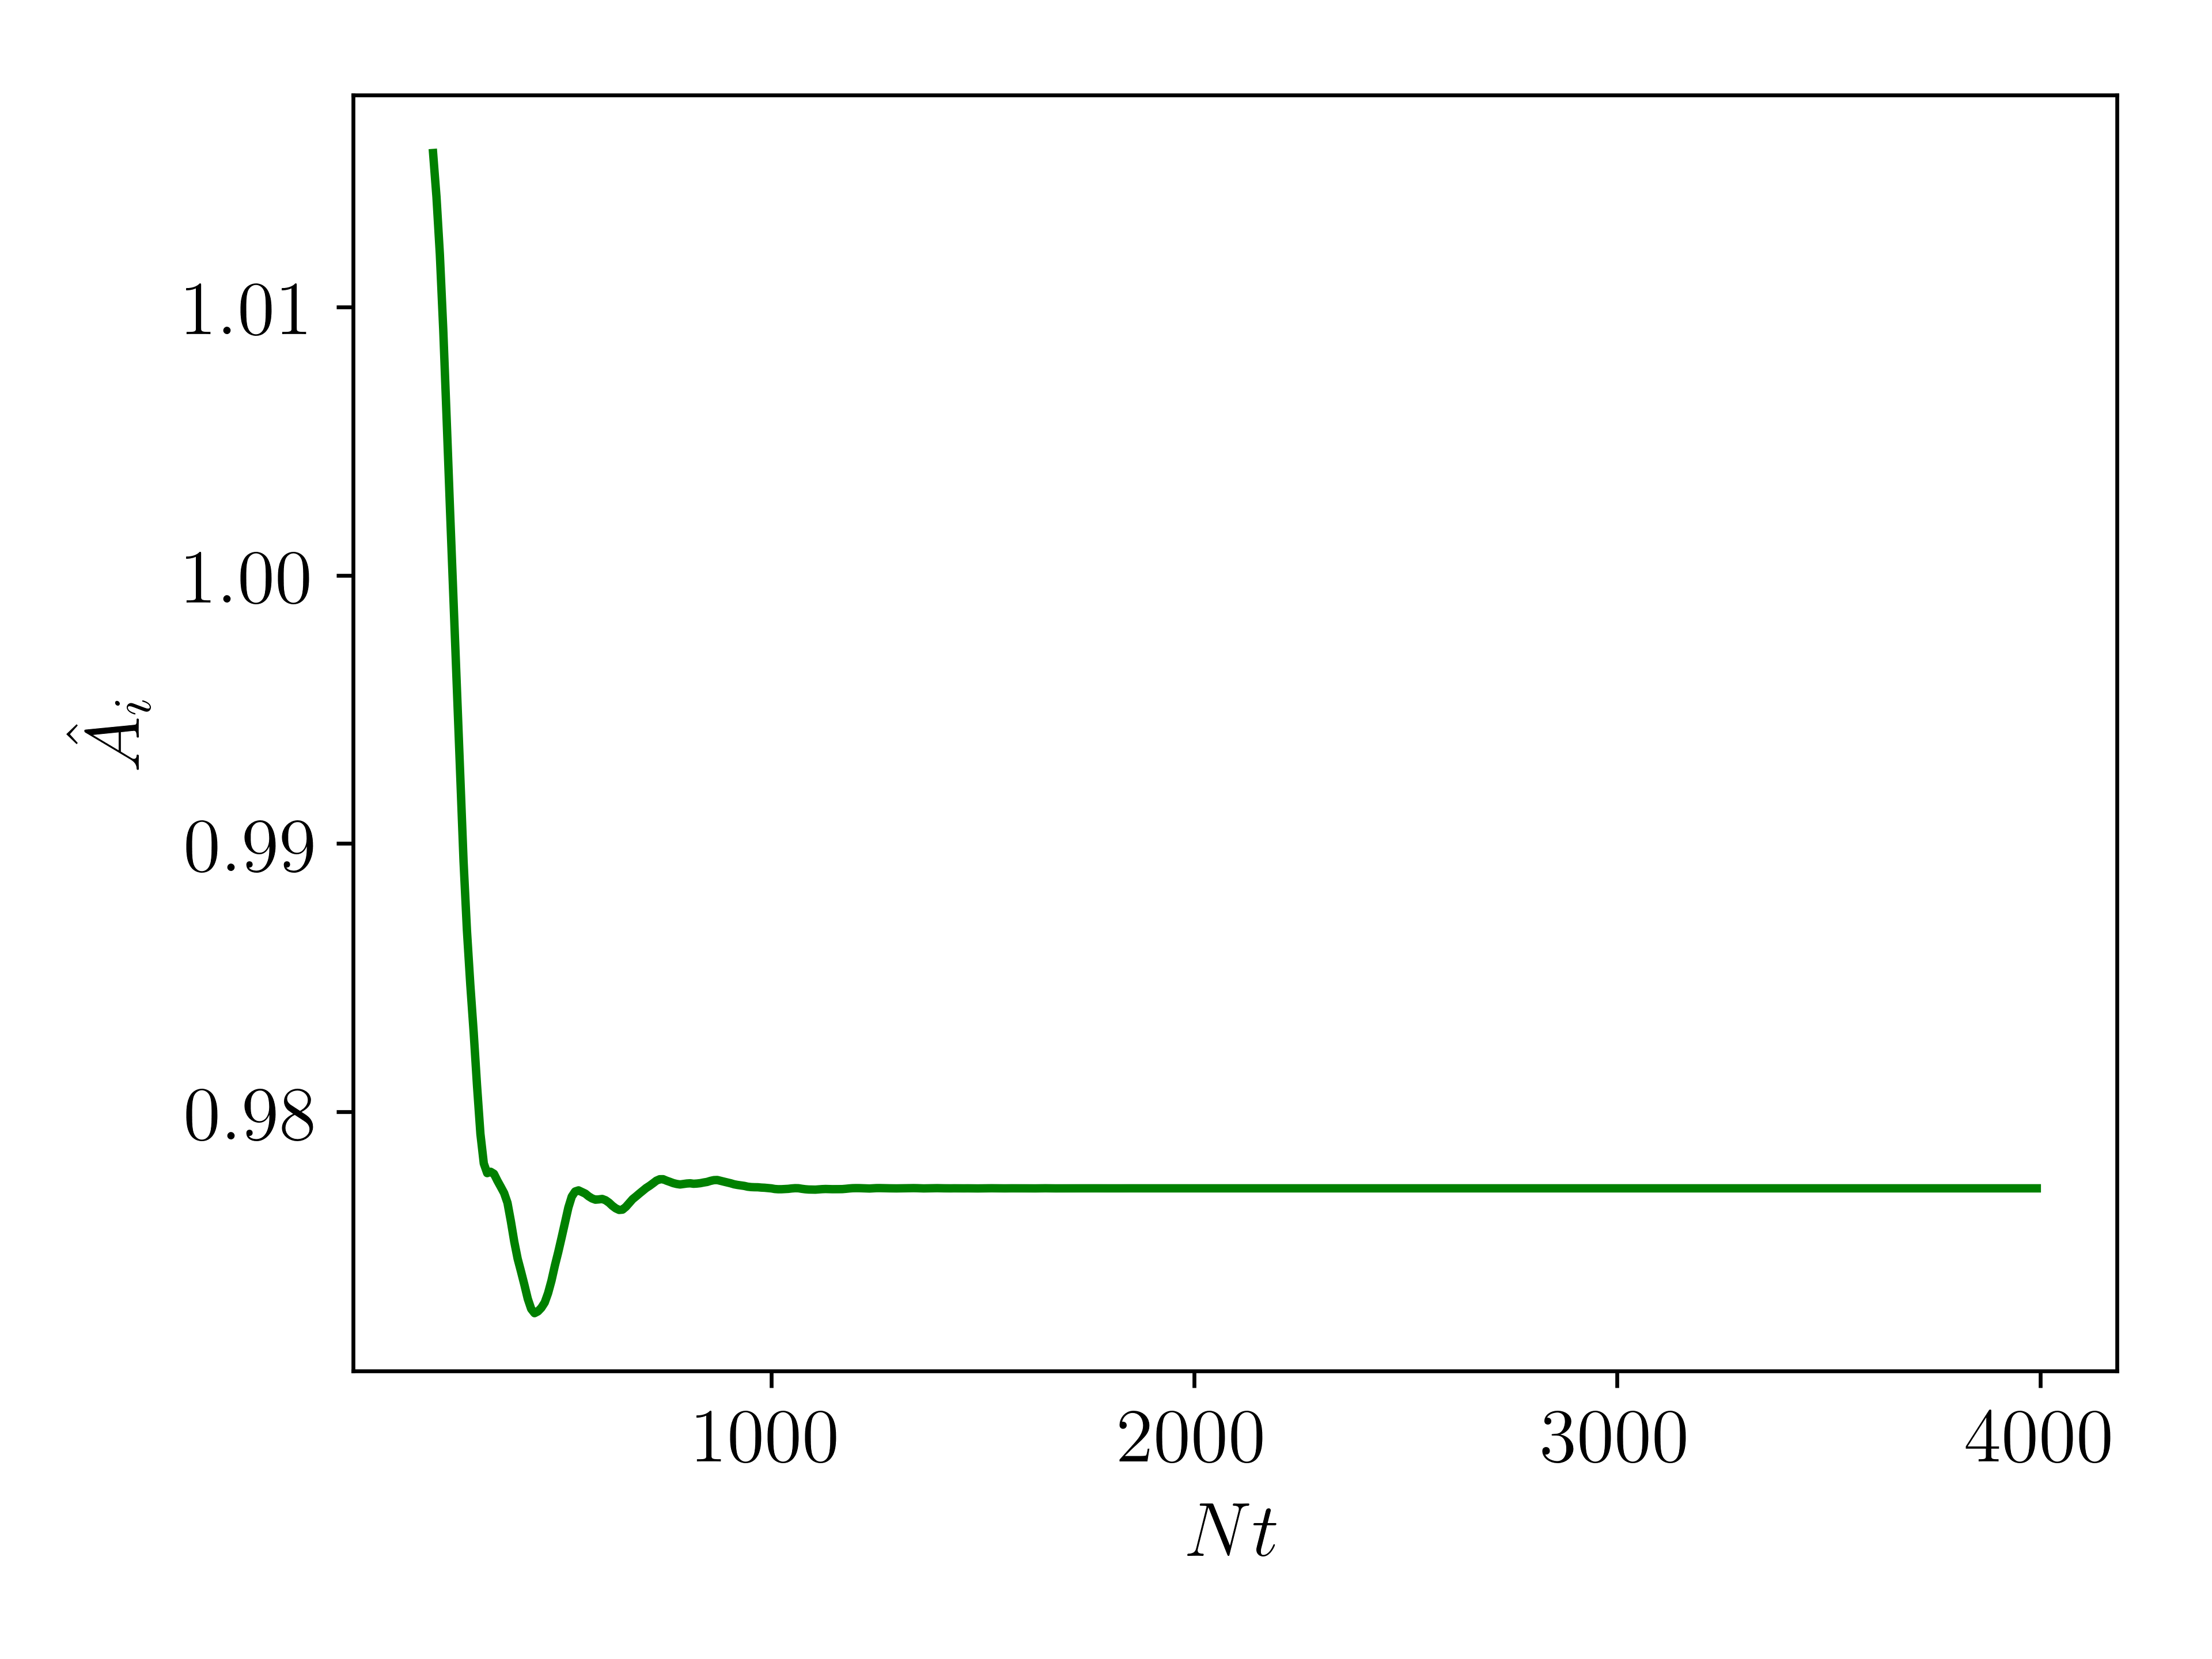
\includegraphics[width=\columnwidth]{plots/lin_amps.png}
    \caption{Amplitude of excited wave over time in weak forcing simulation,
    in units of the analytical estimate \autoref{eq:uz_lin}. We observe great
    agreement with the linear calculation.}\label{fig:lin_amps}
\end{figure}
\begin{figure}[t]
    \centering
    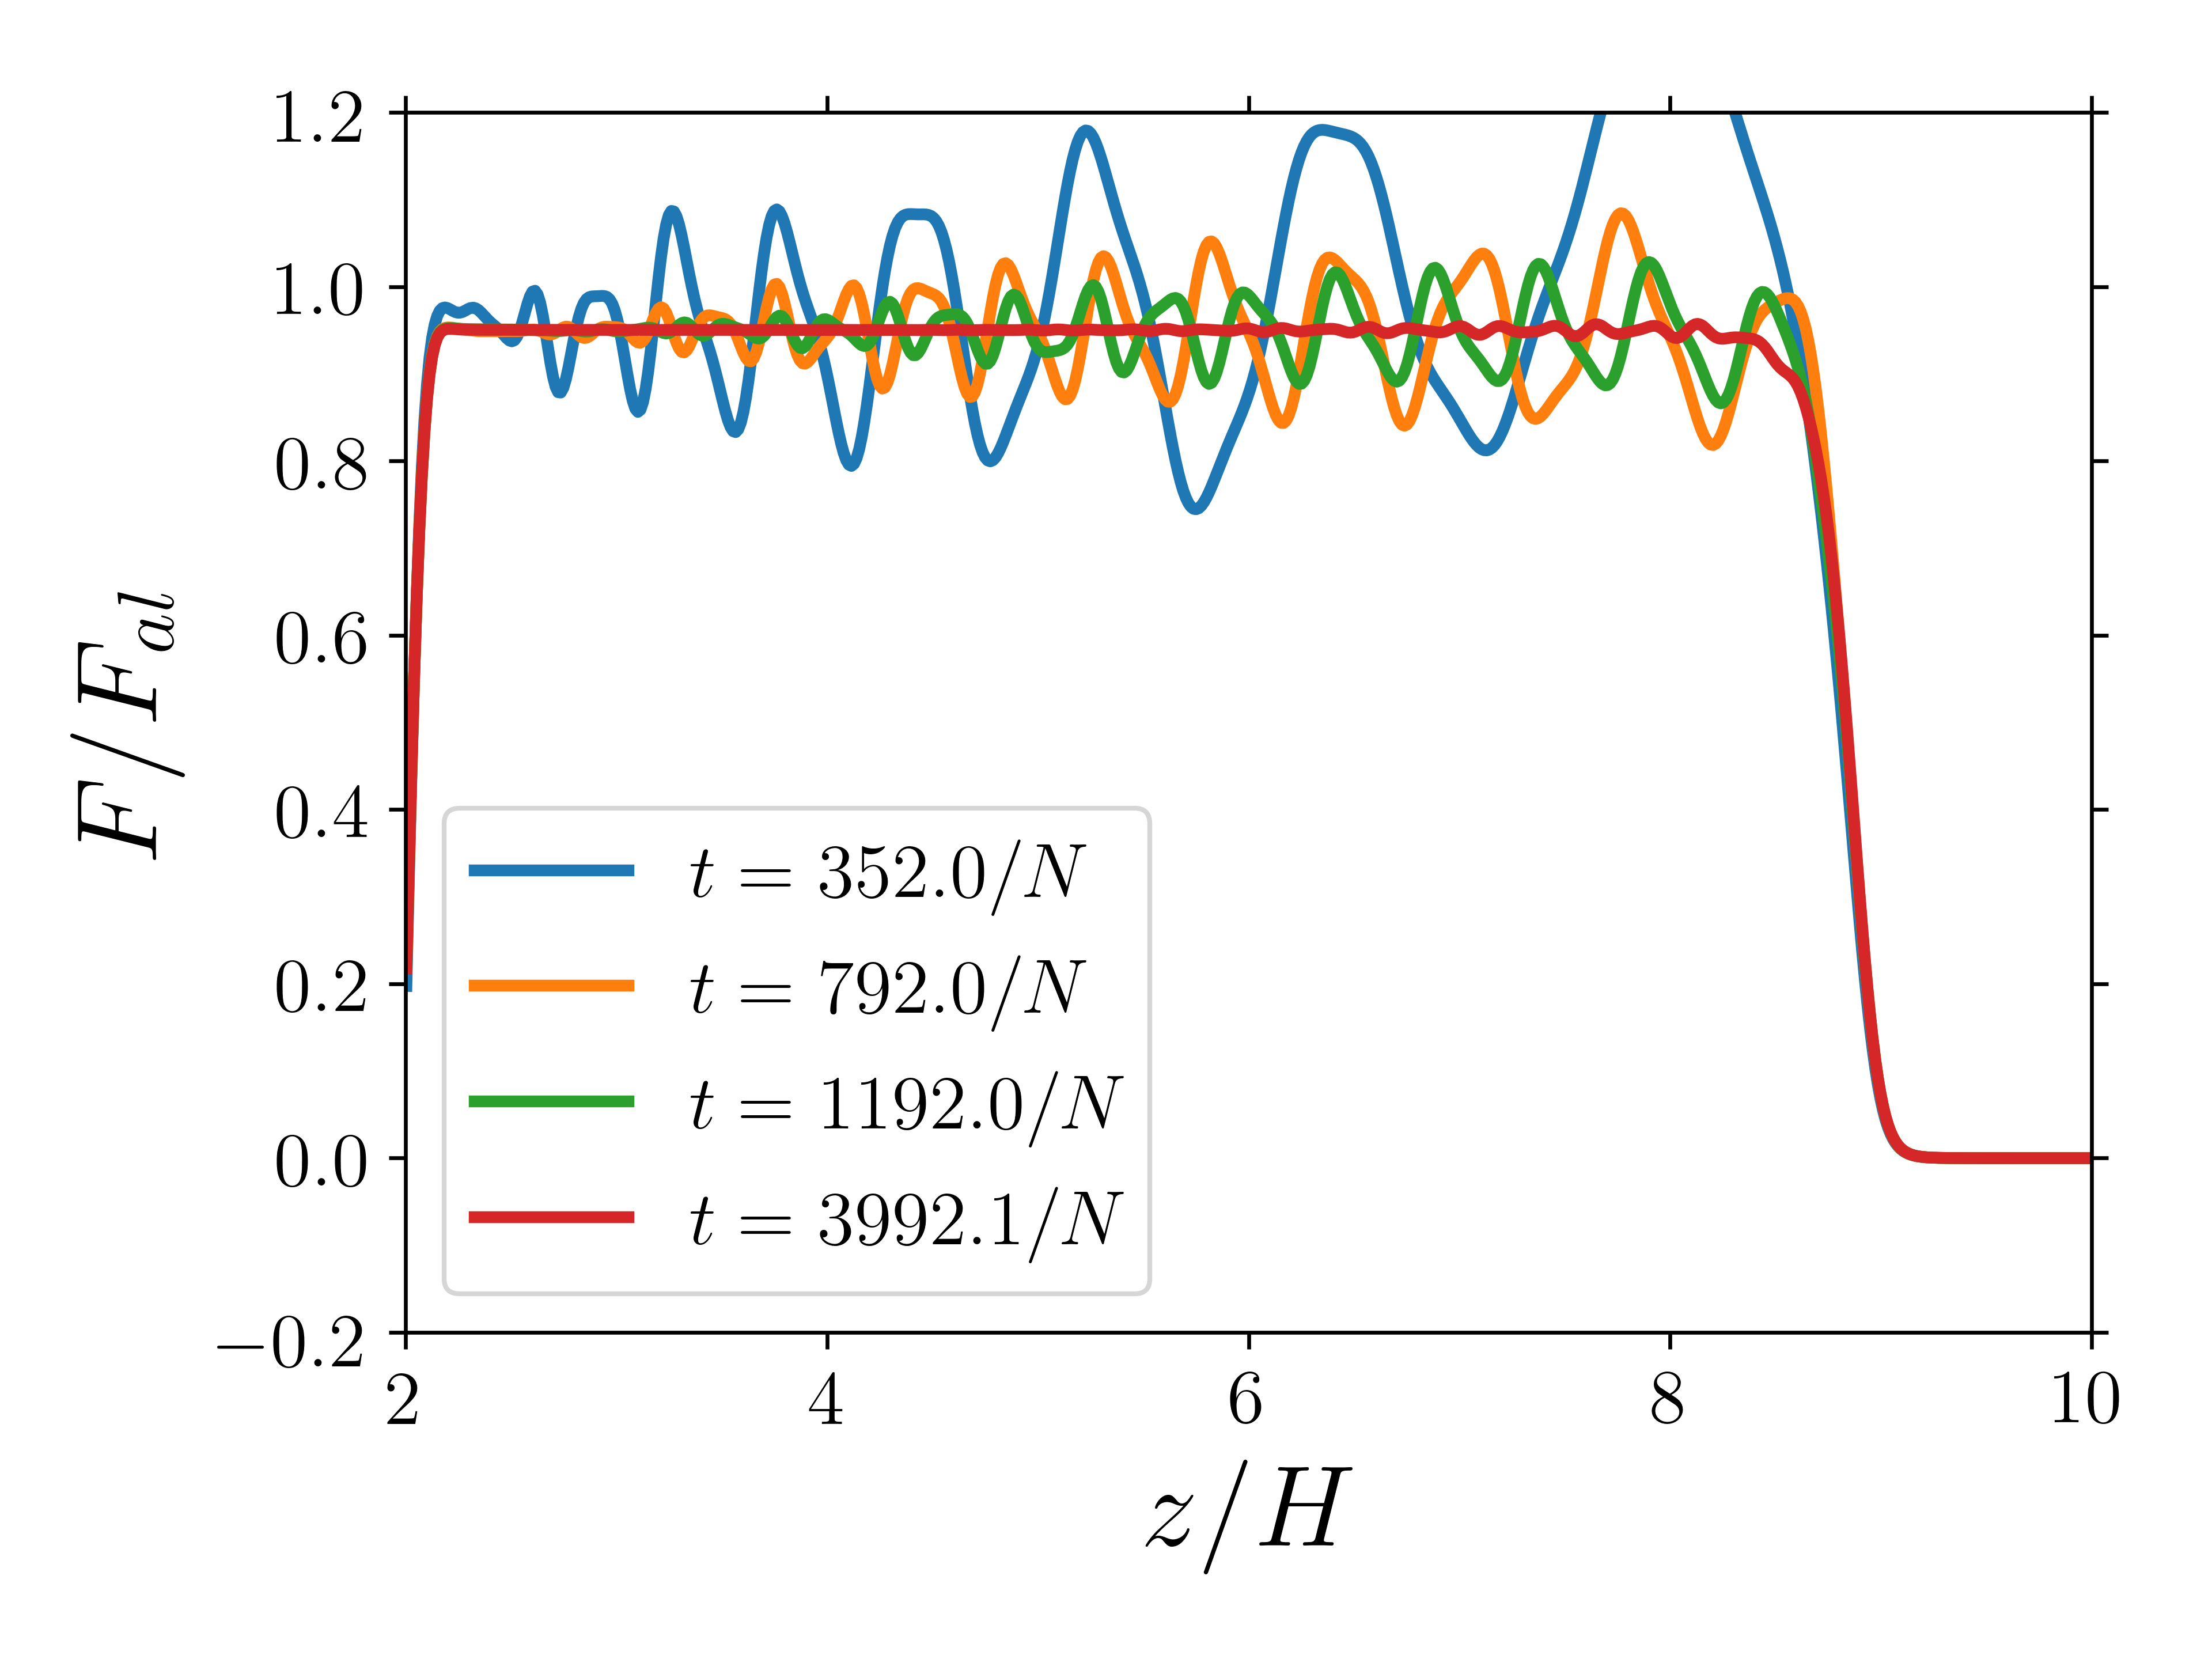
\includegraphics[width=\columnwidth]{plots/lin_fluxes.png}
    \caption{Horizontal momentum flux $S(z, t)$ in units of the analytical estimator
    given by \autoref{eq:S_lin} as a function of $z$ at select times $t$. As
    initial transients die out, the flux converges to be flat below the damping
    layer. The flux excited in the forcing zone is transported without loss to
    the top of the domain, where it is dissipated by the damping layer
    (see \autoref{ss:damping}) without reflection.}\label{fig:lin_fluxes}
\end{figure}

\section{Internal Gravity Waves: Nonlinear Simulation}\label{s:sim}

\subsection{Mean Flow Critical Layer Absorption}

A Navier-Stokes numerical viscosity $\nu$ is used to damp high wavenumbers and
regularize the nonlinear cascade at near grid resolution: $\nu \sim 0.1
\frac{\omega_0}{\abs{k_{0z}}}\frac{L_z}{2\pi N_z}$ was found to be suitable for
$N_z = 2048$.

In past studies of IGWs in WDs (cite Fuller \& Lai), $\xi_z \equiv
\frac{u_z}{\omega_0}$ the Lagrangian fluid displacement was often used towards
wave breaking criterion $k_{0z}\xi_z \gtrsim 1$. We argue that the wave's
self-interaction via its generated mean flow $\bar{U}_0$ induces total
absorption when the mean flow exceeds critical value
\begin{equation}
    \bar{U}_c = \frac{\omega_0}{k_{0x}}.
\end{equation}
This is consistent with the picture put forth in e.g.\ Goldreich and Nicholson
(cite).

A purely horizontal shear flow $\bar{U}_0(z) \hat{x}$ can be seen in
\autoref{se:nl_orig} to have the effect of modifying time derivatives
$\partial_t$ to their frequency in the comoving frame of the fluid $\partial_t -
\bar{U}_0(z)\partial_x$. For a critical value $\omega_0 - \bar{U}_c k_{0x} = 0$,
the frequency of the linear wave in the fluid's frame of reference vanishes and
critical behavior is observed. In a linear theory or a theory where small scales
are viscosity rather than advection dominated, the incident wave has amplitude
reflection and transmission coefficients
\begin{align}
    \mathcal{R} &= e^{-2\pi \sqrt{\mathrm{Ri} - \frac{1}{4}}}, &
    \mathcal{T} &= e^{-\pi \sqrt{\mathrm{Ri} - \frac{1}{4}}},
    \label{eq:crit_coeffs}
\end{align}
where we have defined Richardson number $\mathrm{Ri} \equiv
\at{\frac{N^2}{\p{\pd{\bar{U}_0}{z}}^2}}_{z_c}$ at the critical layer $z_c:
\bar{U}_0(z_c) = \frac{\omega_0}{k_{0x}}$. For most shear flows, $\mathrm{Ri}
\gg 1$ and so $\mathcal{R}, \mathcal{T} \ll 1$ and the incident wave is
absorbed.

When the fluid absorbs the incident wave, it absorbs the incident horizontal
momentum flux as well, which is converted into additional horizontal momentum of
the shear flow. Since the shear flow cannot exceed $\bar{U}_c$ the horizontal
phase velocity of the incident wave, the critical layer must thus propagate
downwards (towards the wave source) to accommodate the incident momentum. In
other words, the total horizontal momentum of the shear flow obeys conservation
equation
\begin{equation}
    \pd{}{t}\int\limits_0^{L_z} \rho(z) \bar{U}_0(z, t)\;\mathrm{d}z
        - \Delta S = 0.
\end{equation}
We define $\Delta S$ to be the change in flux across the critical layer, or
equivalently the absorbed flux. Treating $\bar{U}_0(z > z_c) = \bar{U}_c,
\bar{U}(z < z_c) = 0$ gives us exactly
\begin{equation}
    \rho \bar{U}_c\pd{z_c}{t} = -\Delta S.\label{eq:zc_anal}
\end{equation}
For constant $\Delta S$ in space and $\rho \approx \rho_0$, this has analytical
solution
\begin{equation}
    z(t) = -H\ln t - H\ln \frac{H\rho_0(z = 0)c_{ph, x}}{\Delta S}
        .\label{eq:zc_sol}
\end{equation}

\subsection{Numerical Simulation}\label{ss:nl_ns}

We use the same $k_{0x}, \omega_0$ as \autoref{ss:lin_ns}. Our other parameters
are:
\begin{itemize}
    \item We choose $\nu = 0.1 \frac{\omega_0}{k_{0z}k_{z, \max}}$, where
        $k_{z, \max} = \frac{2\pi N_z}{L_z}$. Note that $\nu =
        \frac{\omega_0}{k_{0z} k_{z, \max}}$ corresponds to the advective term
        $\vec{u} \cdot \vec{\nabla}$ being of the same order as the time
        derivative $\partial_t$ for flow velocities $\vec{u} \sim
        \frac{\omega_0}{k_{0z}}$ at the grid spacing.
\end{itemize}

Two representative snapshots from our simulation are provided in
TODO after the critical layer has had time to form. We may note that
the critical layer, where $S_{px}$ is absorbed and $\bar{U}_0 = \bar{U}_c$,
travels downwards as predicted.

\subsection{Propagating Critical Layer}

For the simulation in TODO, we may define $z_c = \argmax_z
\pd{\bar{U}_0}{z}$. Computing $\pd{z_c}{t}$ using the analytical flux
\autoref{eq:S_lin} allows comparison to \autoref{eq:zc_anal}, which we exhibit
in TODO\@. We see overall good agreement, though some small
deviation is expected since $S_{px}$ is not perfectly conserved owing to
numerical viscosity (and YUBONOTE $S_{px}$ is misestimated?).

However, recalling \autoref{eq:crit_coeffs}, we only expect complete critical
layer absorption when $\mathrm{Ri} \gg \frac{1}{4}$. We may plot $\mathrm{Ri}$
over the same time interval in TODO\@. We may observe that the
Richardson number is initially decreasing but eventually levels out and
begins to increase again. This corresponds to an increasingly sharp critical
layer transition then subsequently a decreasingly sharp critical layer
transition.

We argue that the Richardson number is bounded from below by viscosity. A
repeated simulation with a larger viscosity is shown in TODO,
where the Richardson number does not go nearly as low.

\begin{figure}[t]
    \centering
    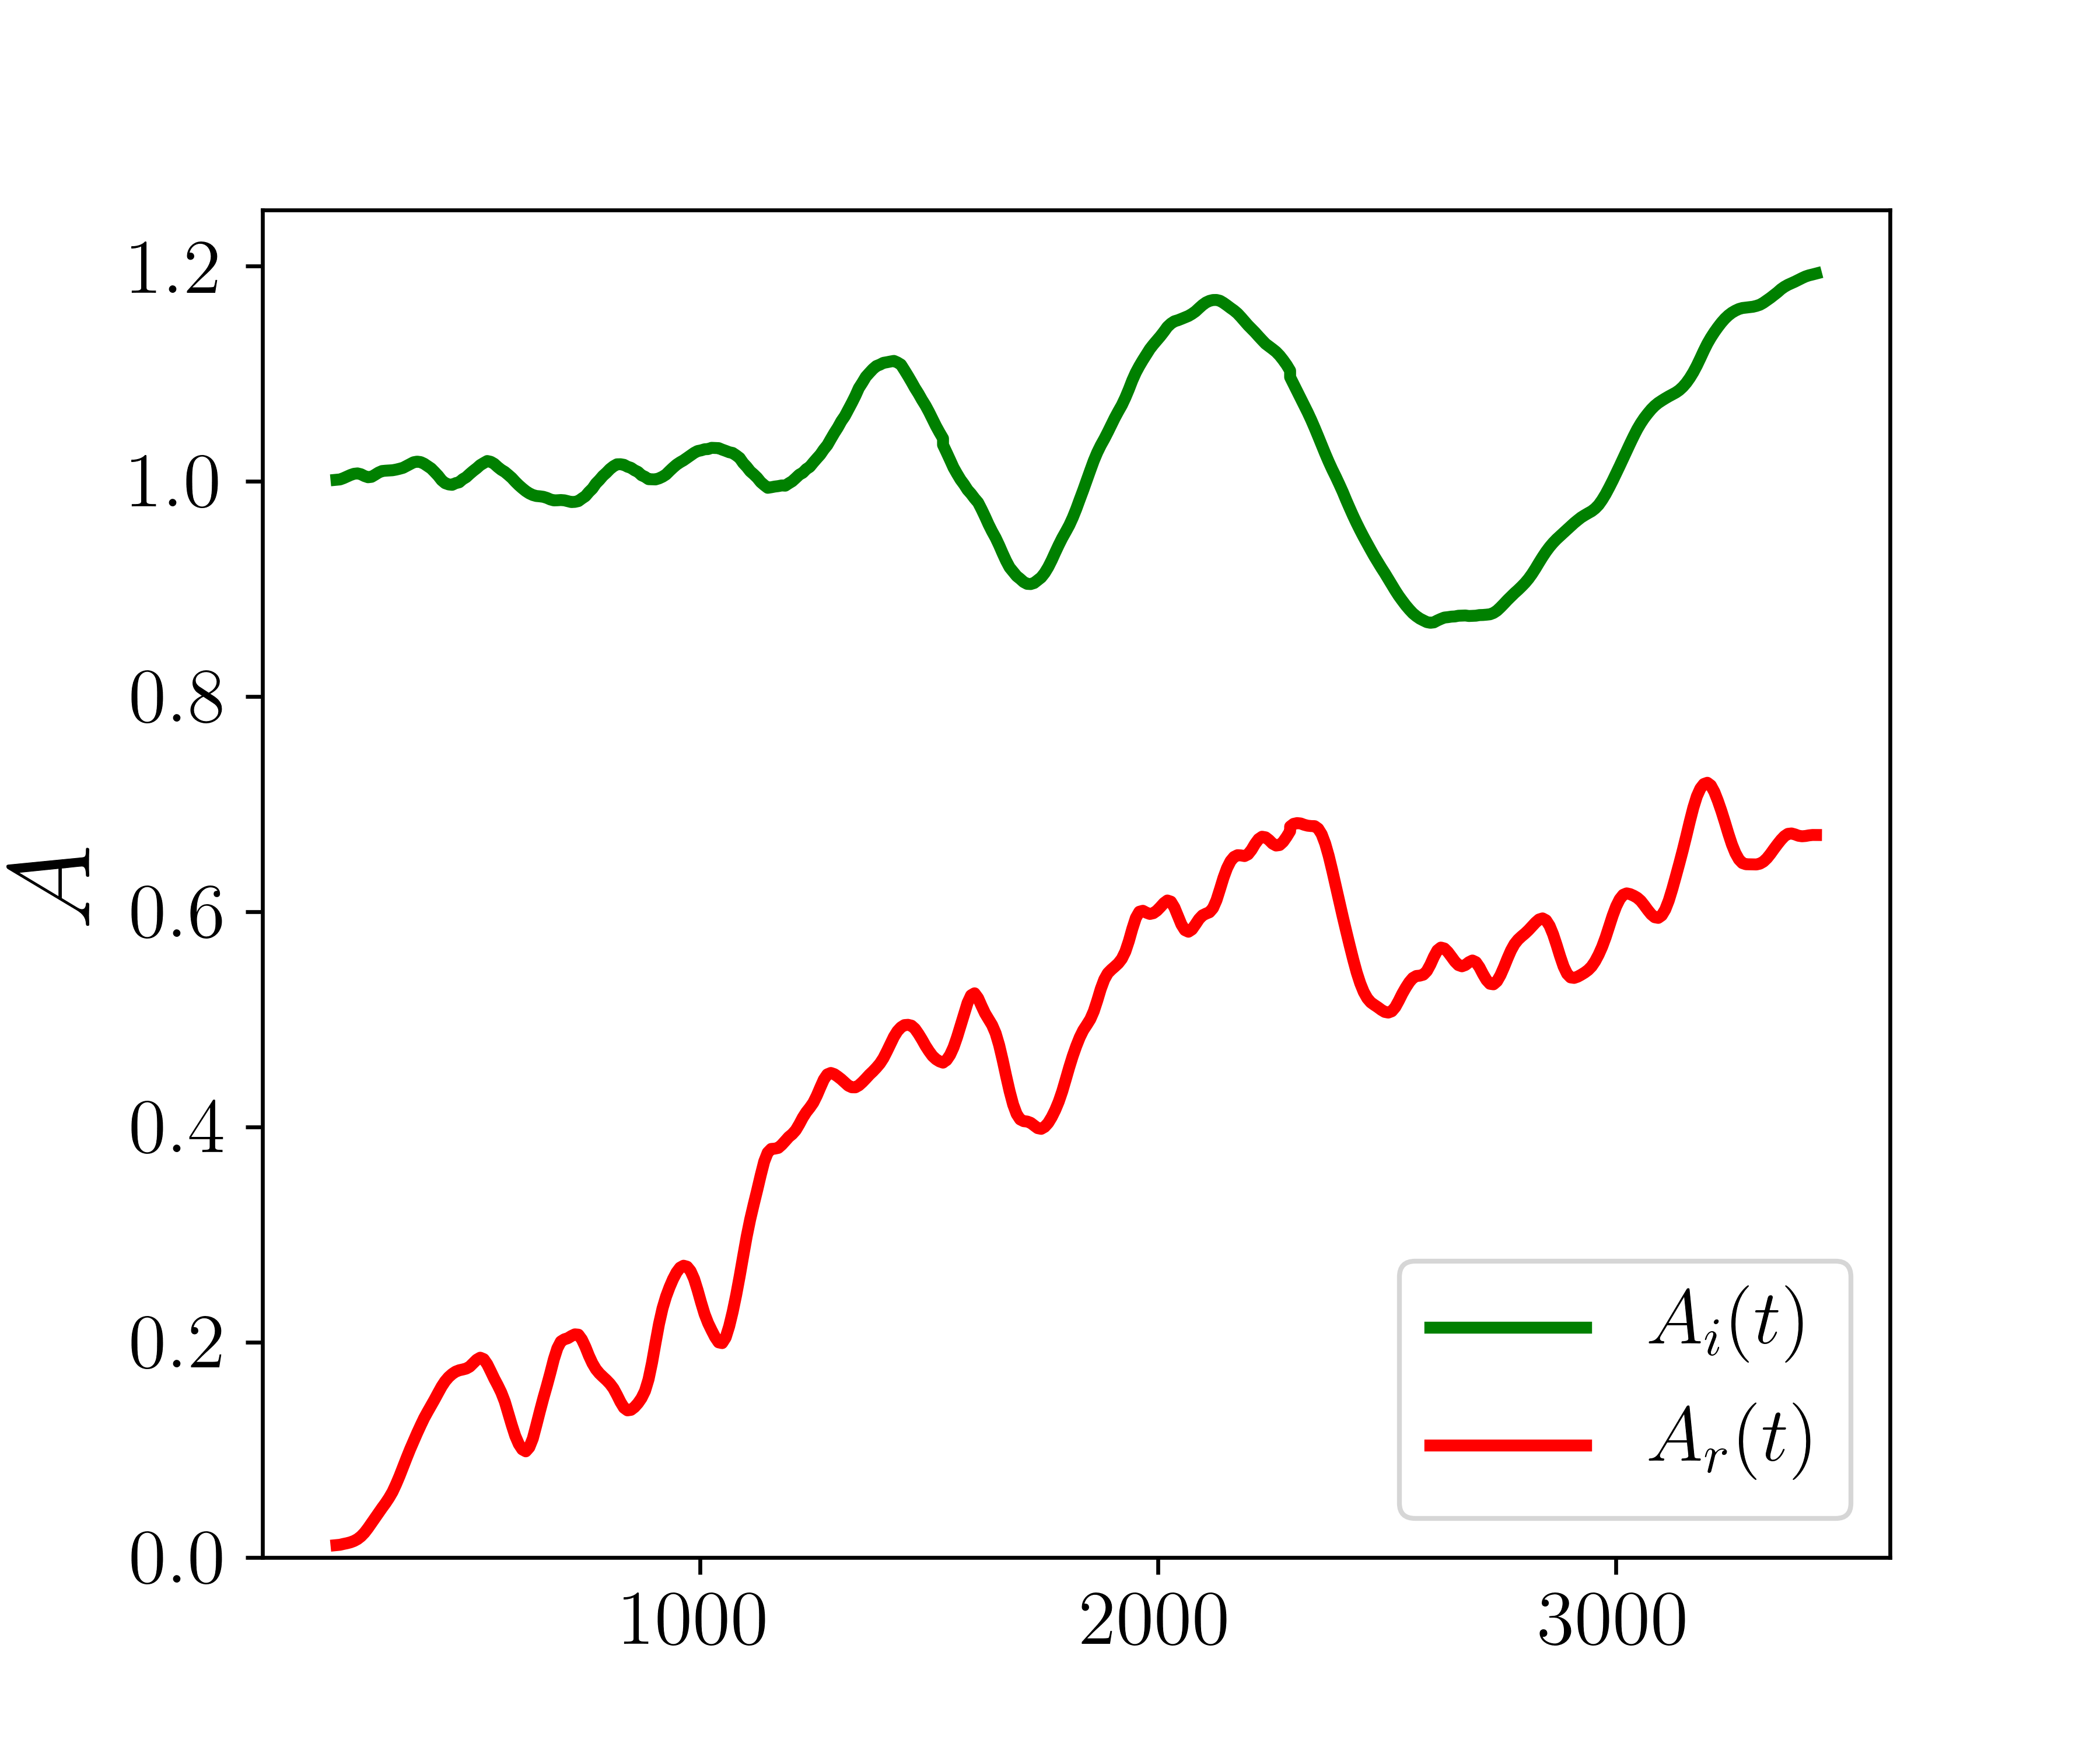
\includegraphics[width=\columnwidth]{plots/nl_f_amps.png}
    \caption{The top panel measures the incident wave amplitude $A_i(t)$ (green)
    and the downwards propagating wave amplitude $A_d(t)$ (red) just above the
    forcing zone, normalized to the analytical estimate \autoref{eq:uz_lin}.
    $A_d \neq 0$ due to reflection off the critical layer. The bottom panel
    shows the behavior of three horizontal momentum fluxes over time, in units
    of the analytical estimate \autoref{eq:S_lin}: (blue) flux incident on the
    critical layer, (black) flux absorbed by the critical layer, and (green)
    flux transmitted through the critical layer. A fiducial simulation of
    $\mathrm{Re} = 1000$ is shown.}\label{fig:nl_amps}
\end{figure}

\begin{figure}[t]
    \centering
    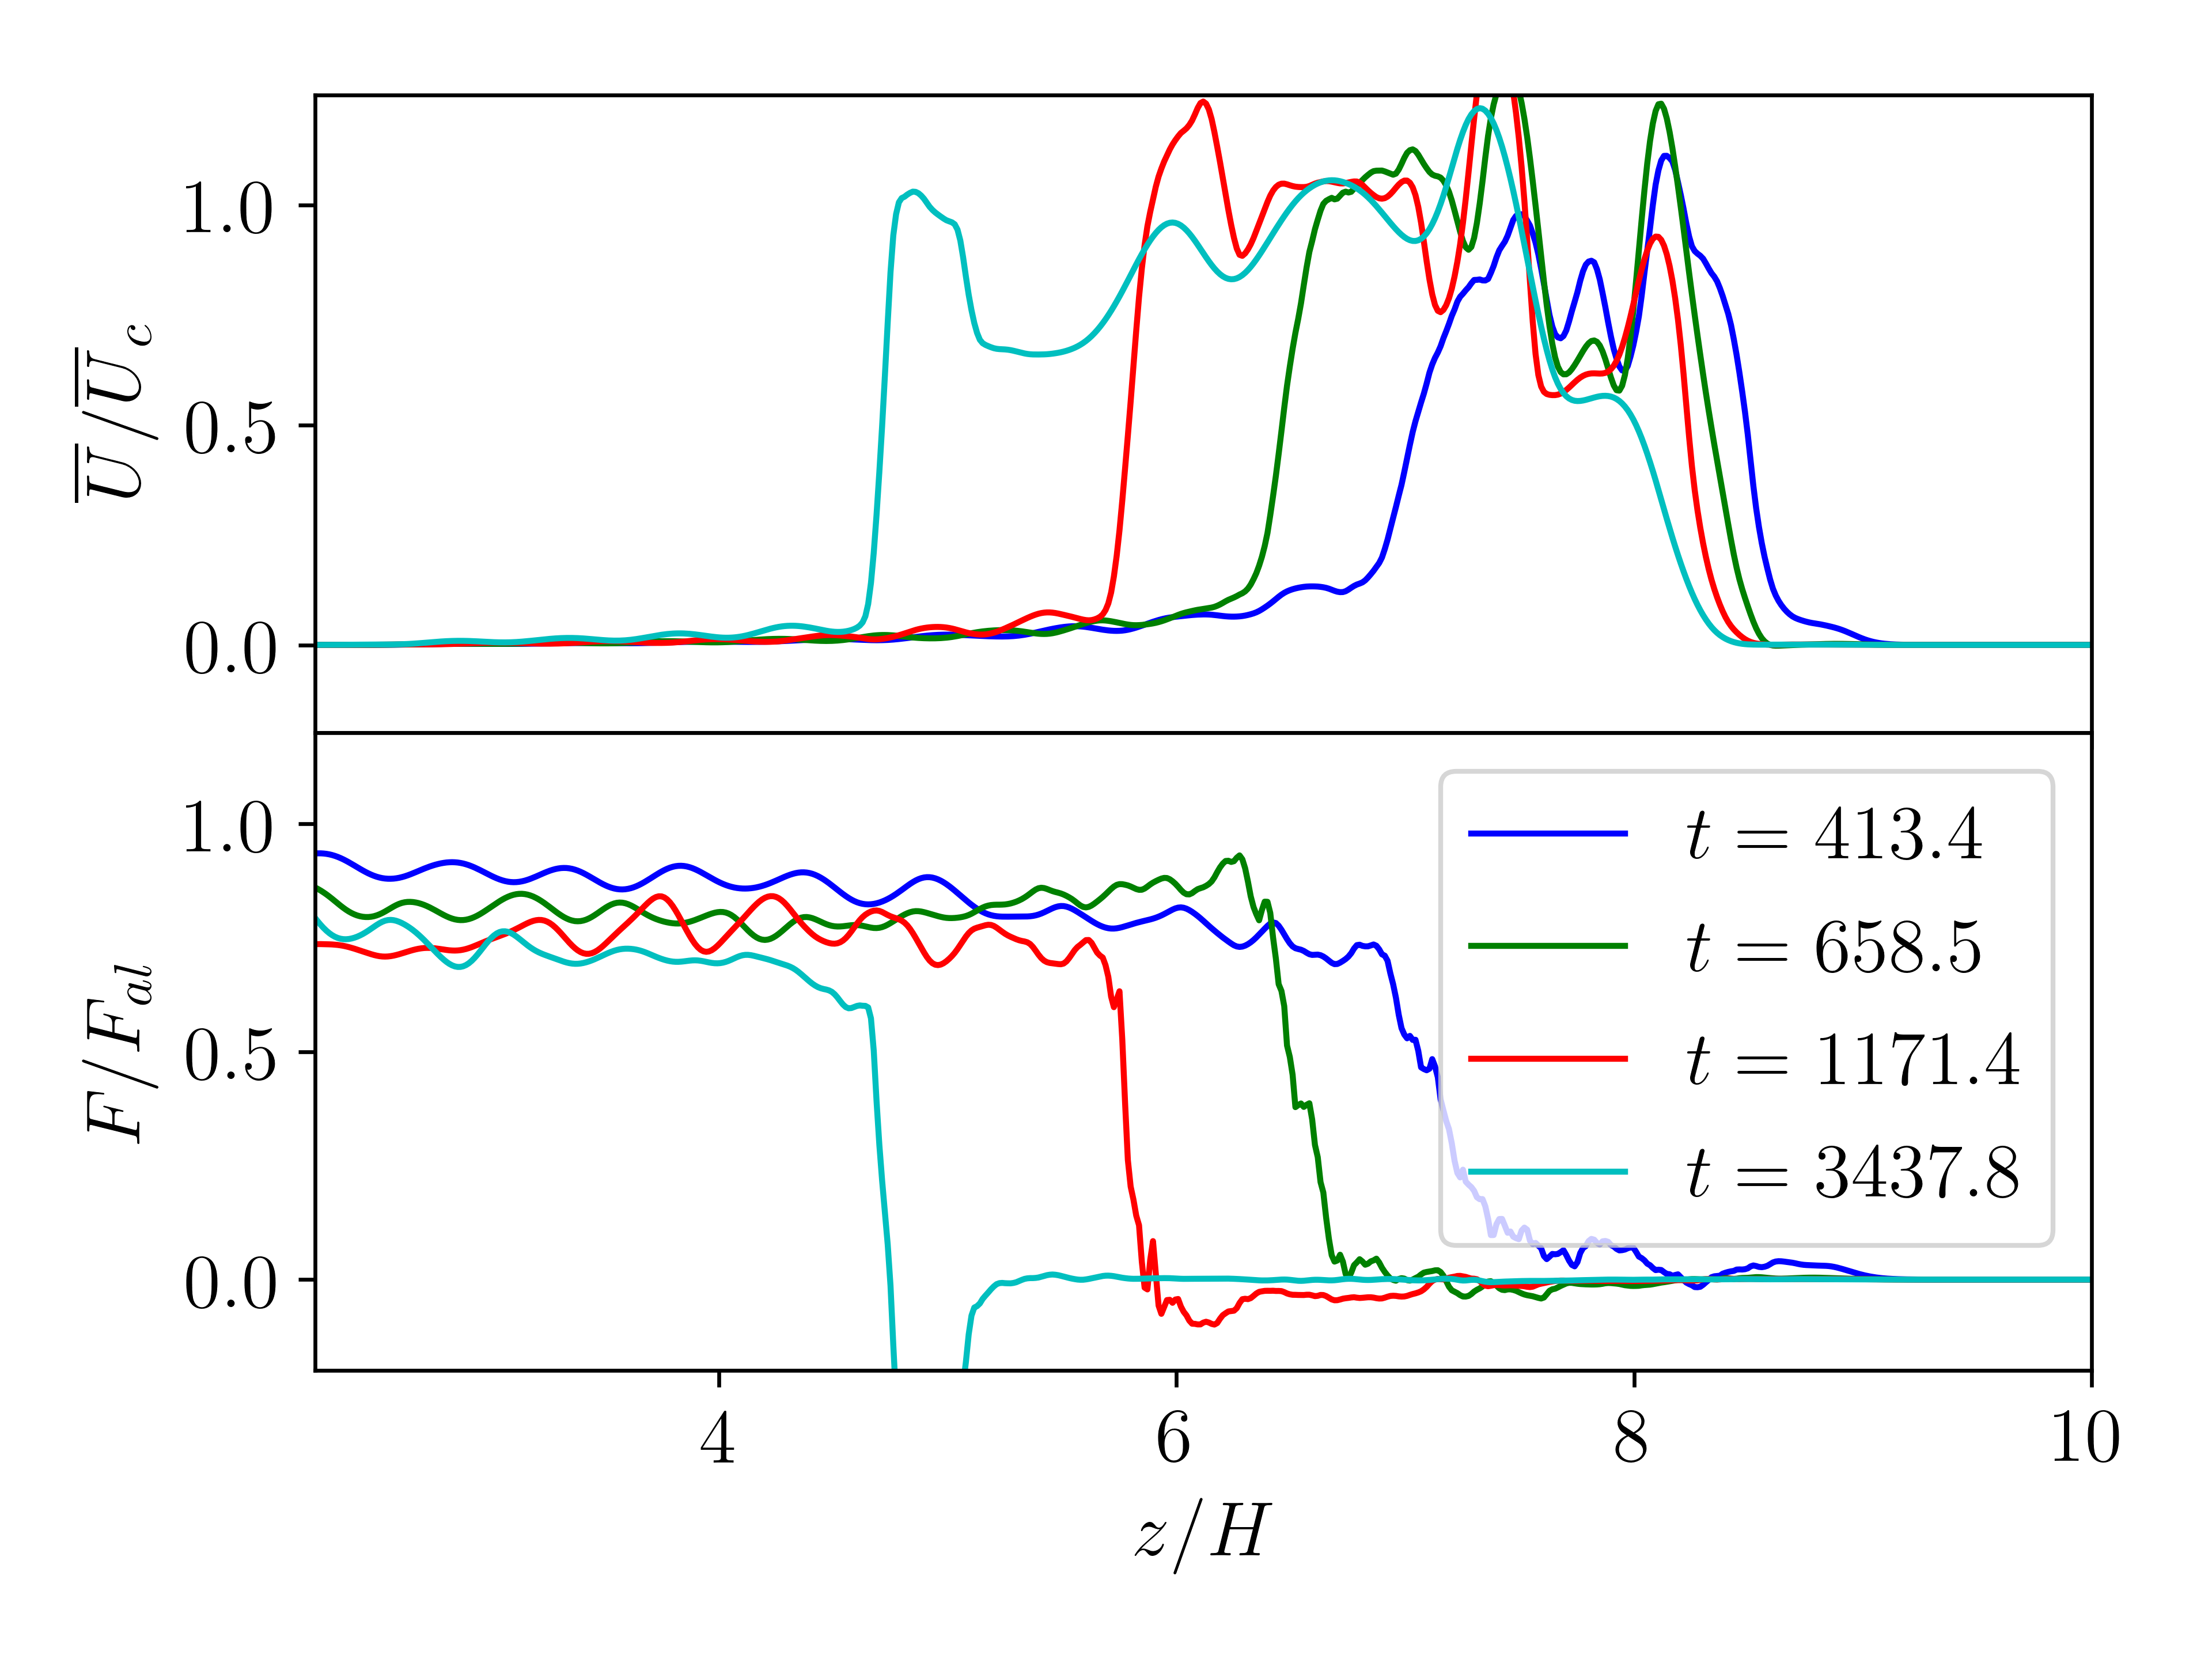
\includegraphics[width=\columnwidth]{plots/nl_fluxes.png}
    \caption{The top and bottom panels show respectively the mean flow
    $\bar{U}_0$ (see \autoref{eq:mean_flow}) and horizontal momentum flux $S$
    (see \autoref{eq:S_def}) as a function of $z$ at certain times $t$. The same
    color coding is used for the two plots. The mean flow is normalized to its
    critical value $c_{ph,x}$ while again $S$ is normalized to its analytical
    estimate \autoref{eq:S_lin}.}\label{fig:nl_fluxes}
\end{figure}

\begin{figure}[t]
    \centering
    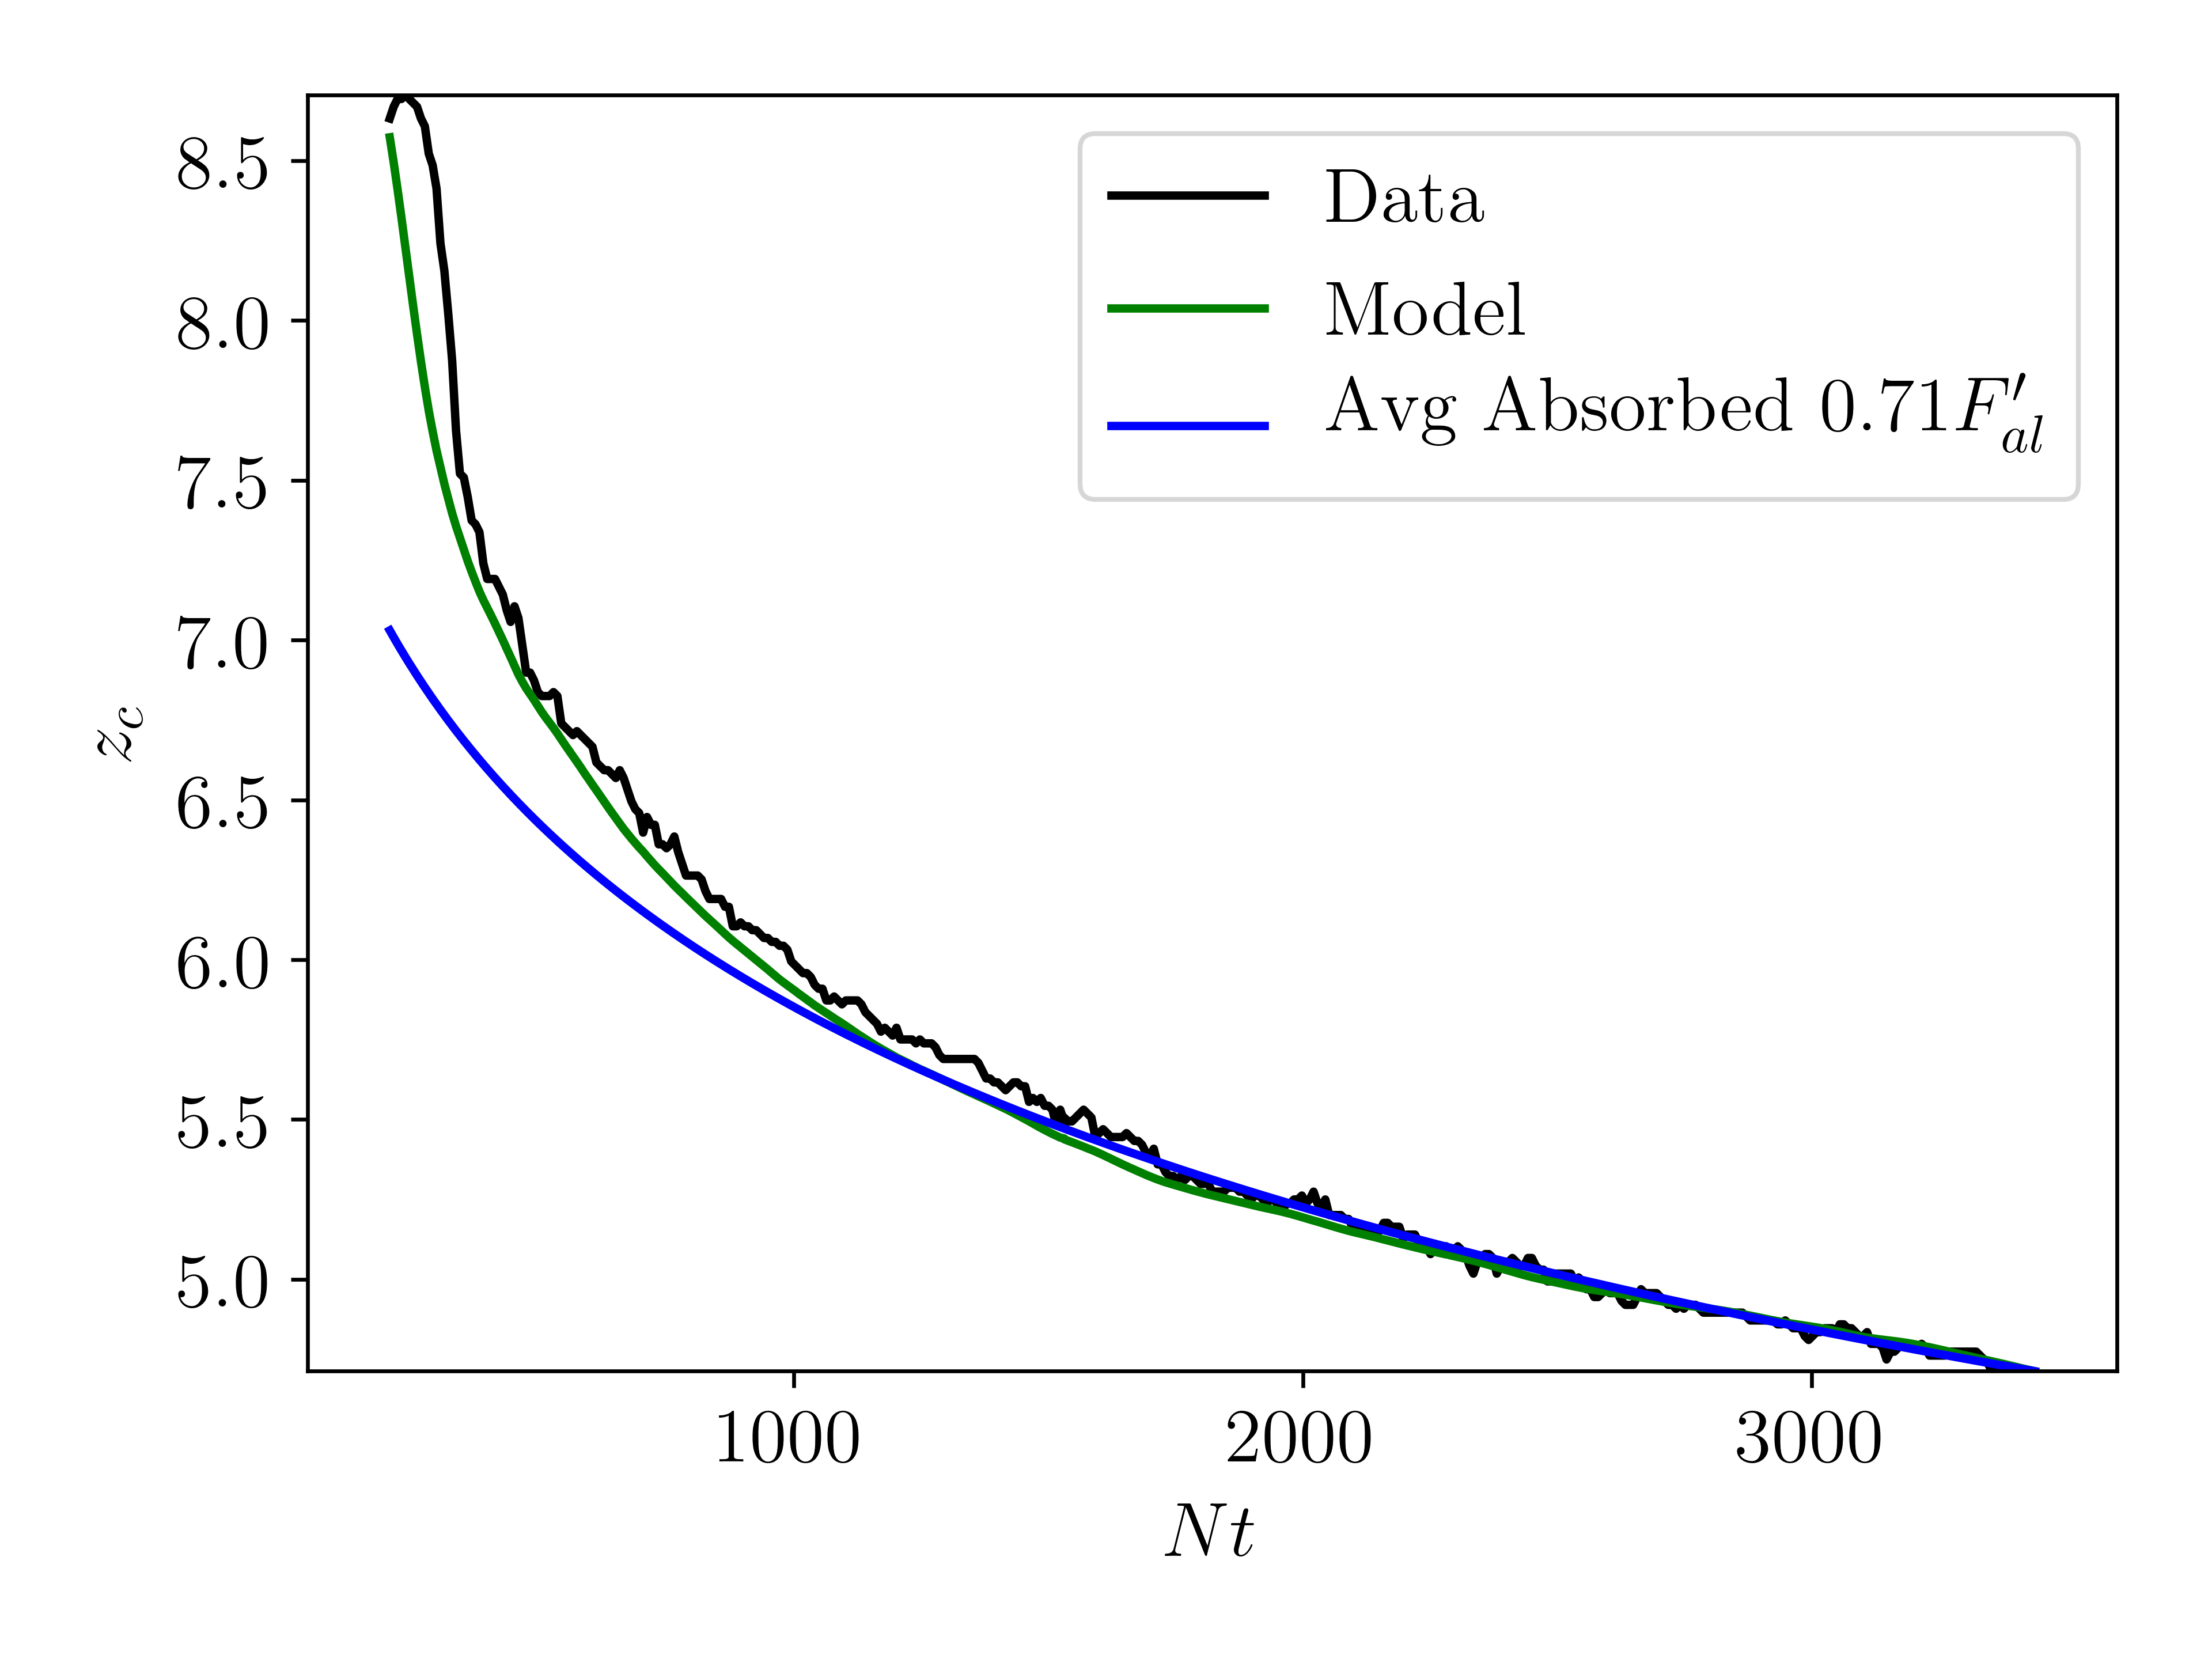
\includegraphics[width=\columnwidth]{plots/nl_front.png}
    \caption{Shown is the position of the critical layer (black) as well as two
    predictors of the critical layer location using the absorbed flux (see the
    second panel of \autoref{fig:nl_amps}). The green line is generated by
    integrating \autoref{eq:zc_anal} using $\Delta S$ from the data, while the
    blue line is generated by using the average value of $\Delta S$ in
    \autoref{eq:zc_sol}.}\label{fig:nl_front}
\end{figure}

\begin{figure}[t]
    \centering
    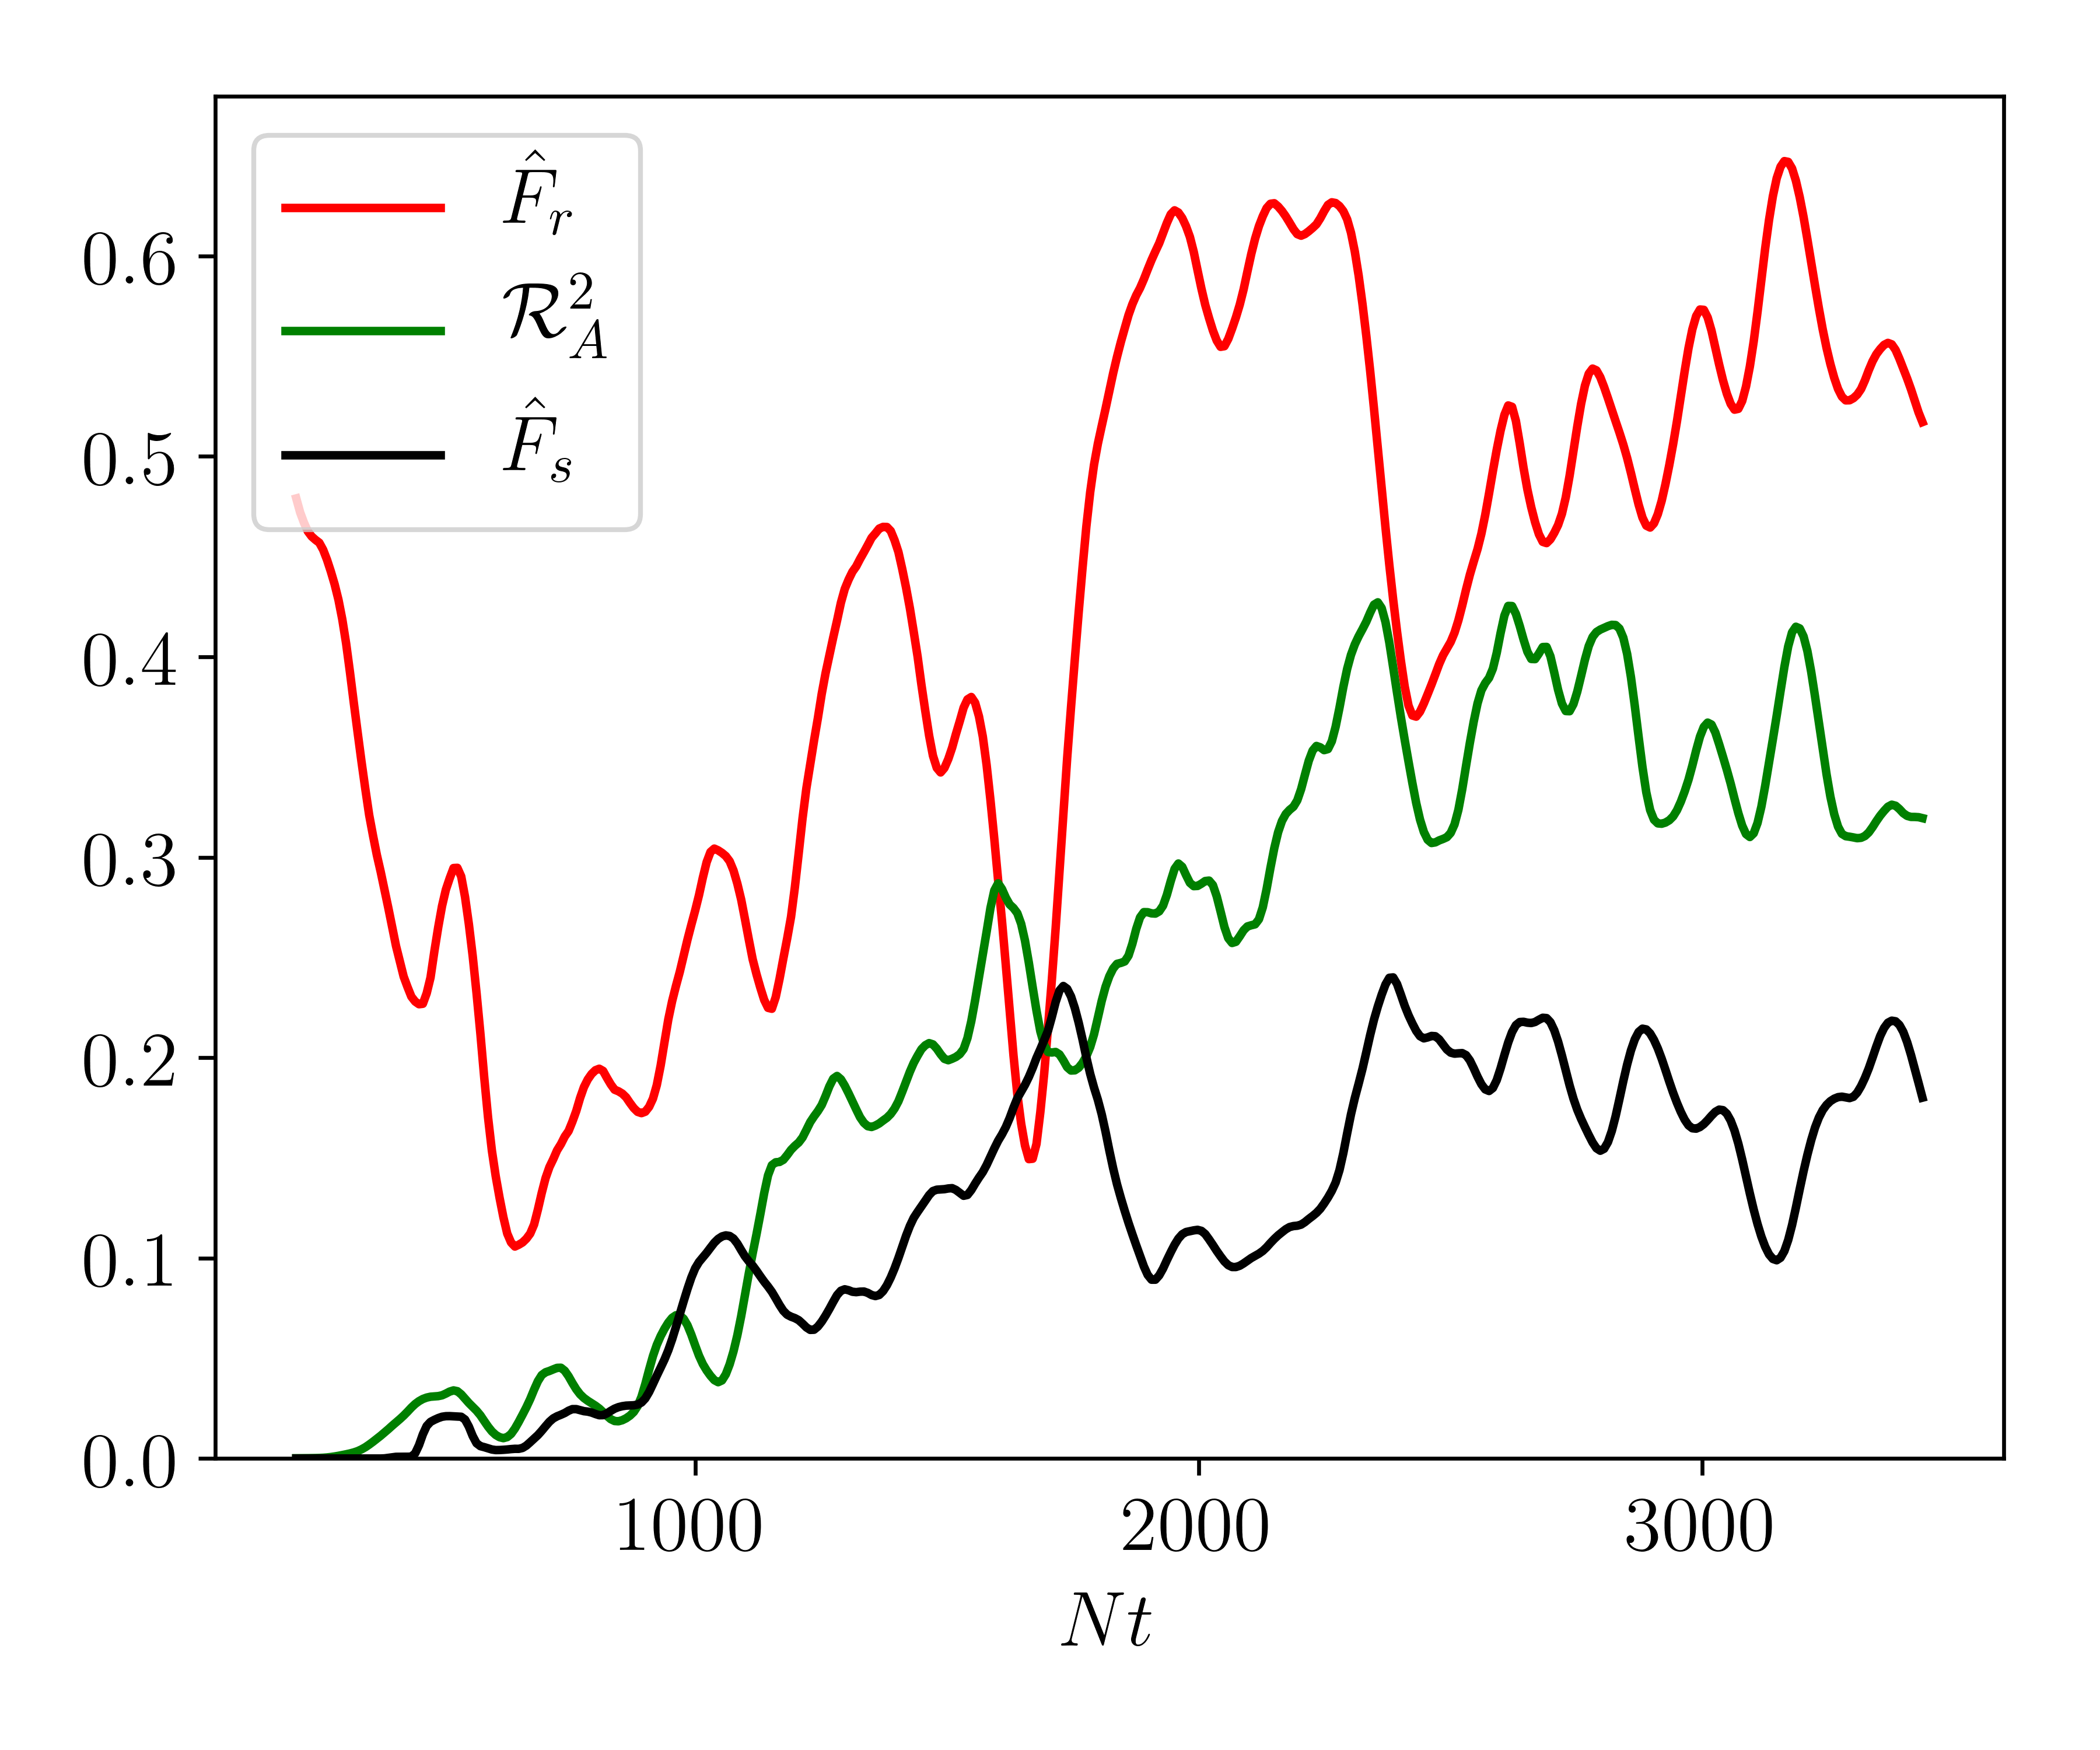
\includegraphics[width=\columnwidth]{plots/nl_f_refl.png}
    \caption{NL reflectivity}\label{fig:nl_refl}
\end{figure}

\section{Discussion}\label{s:discussion}

\begin{figure}[t]
    \centering
    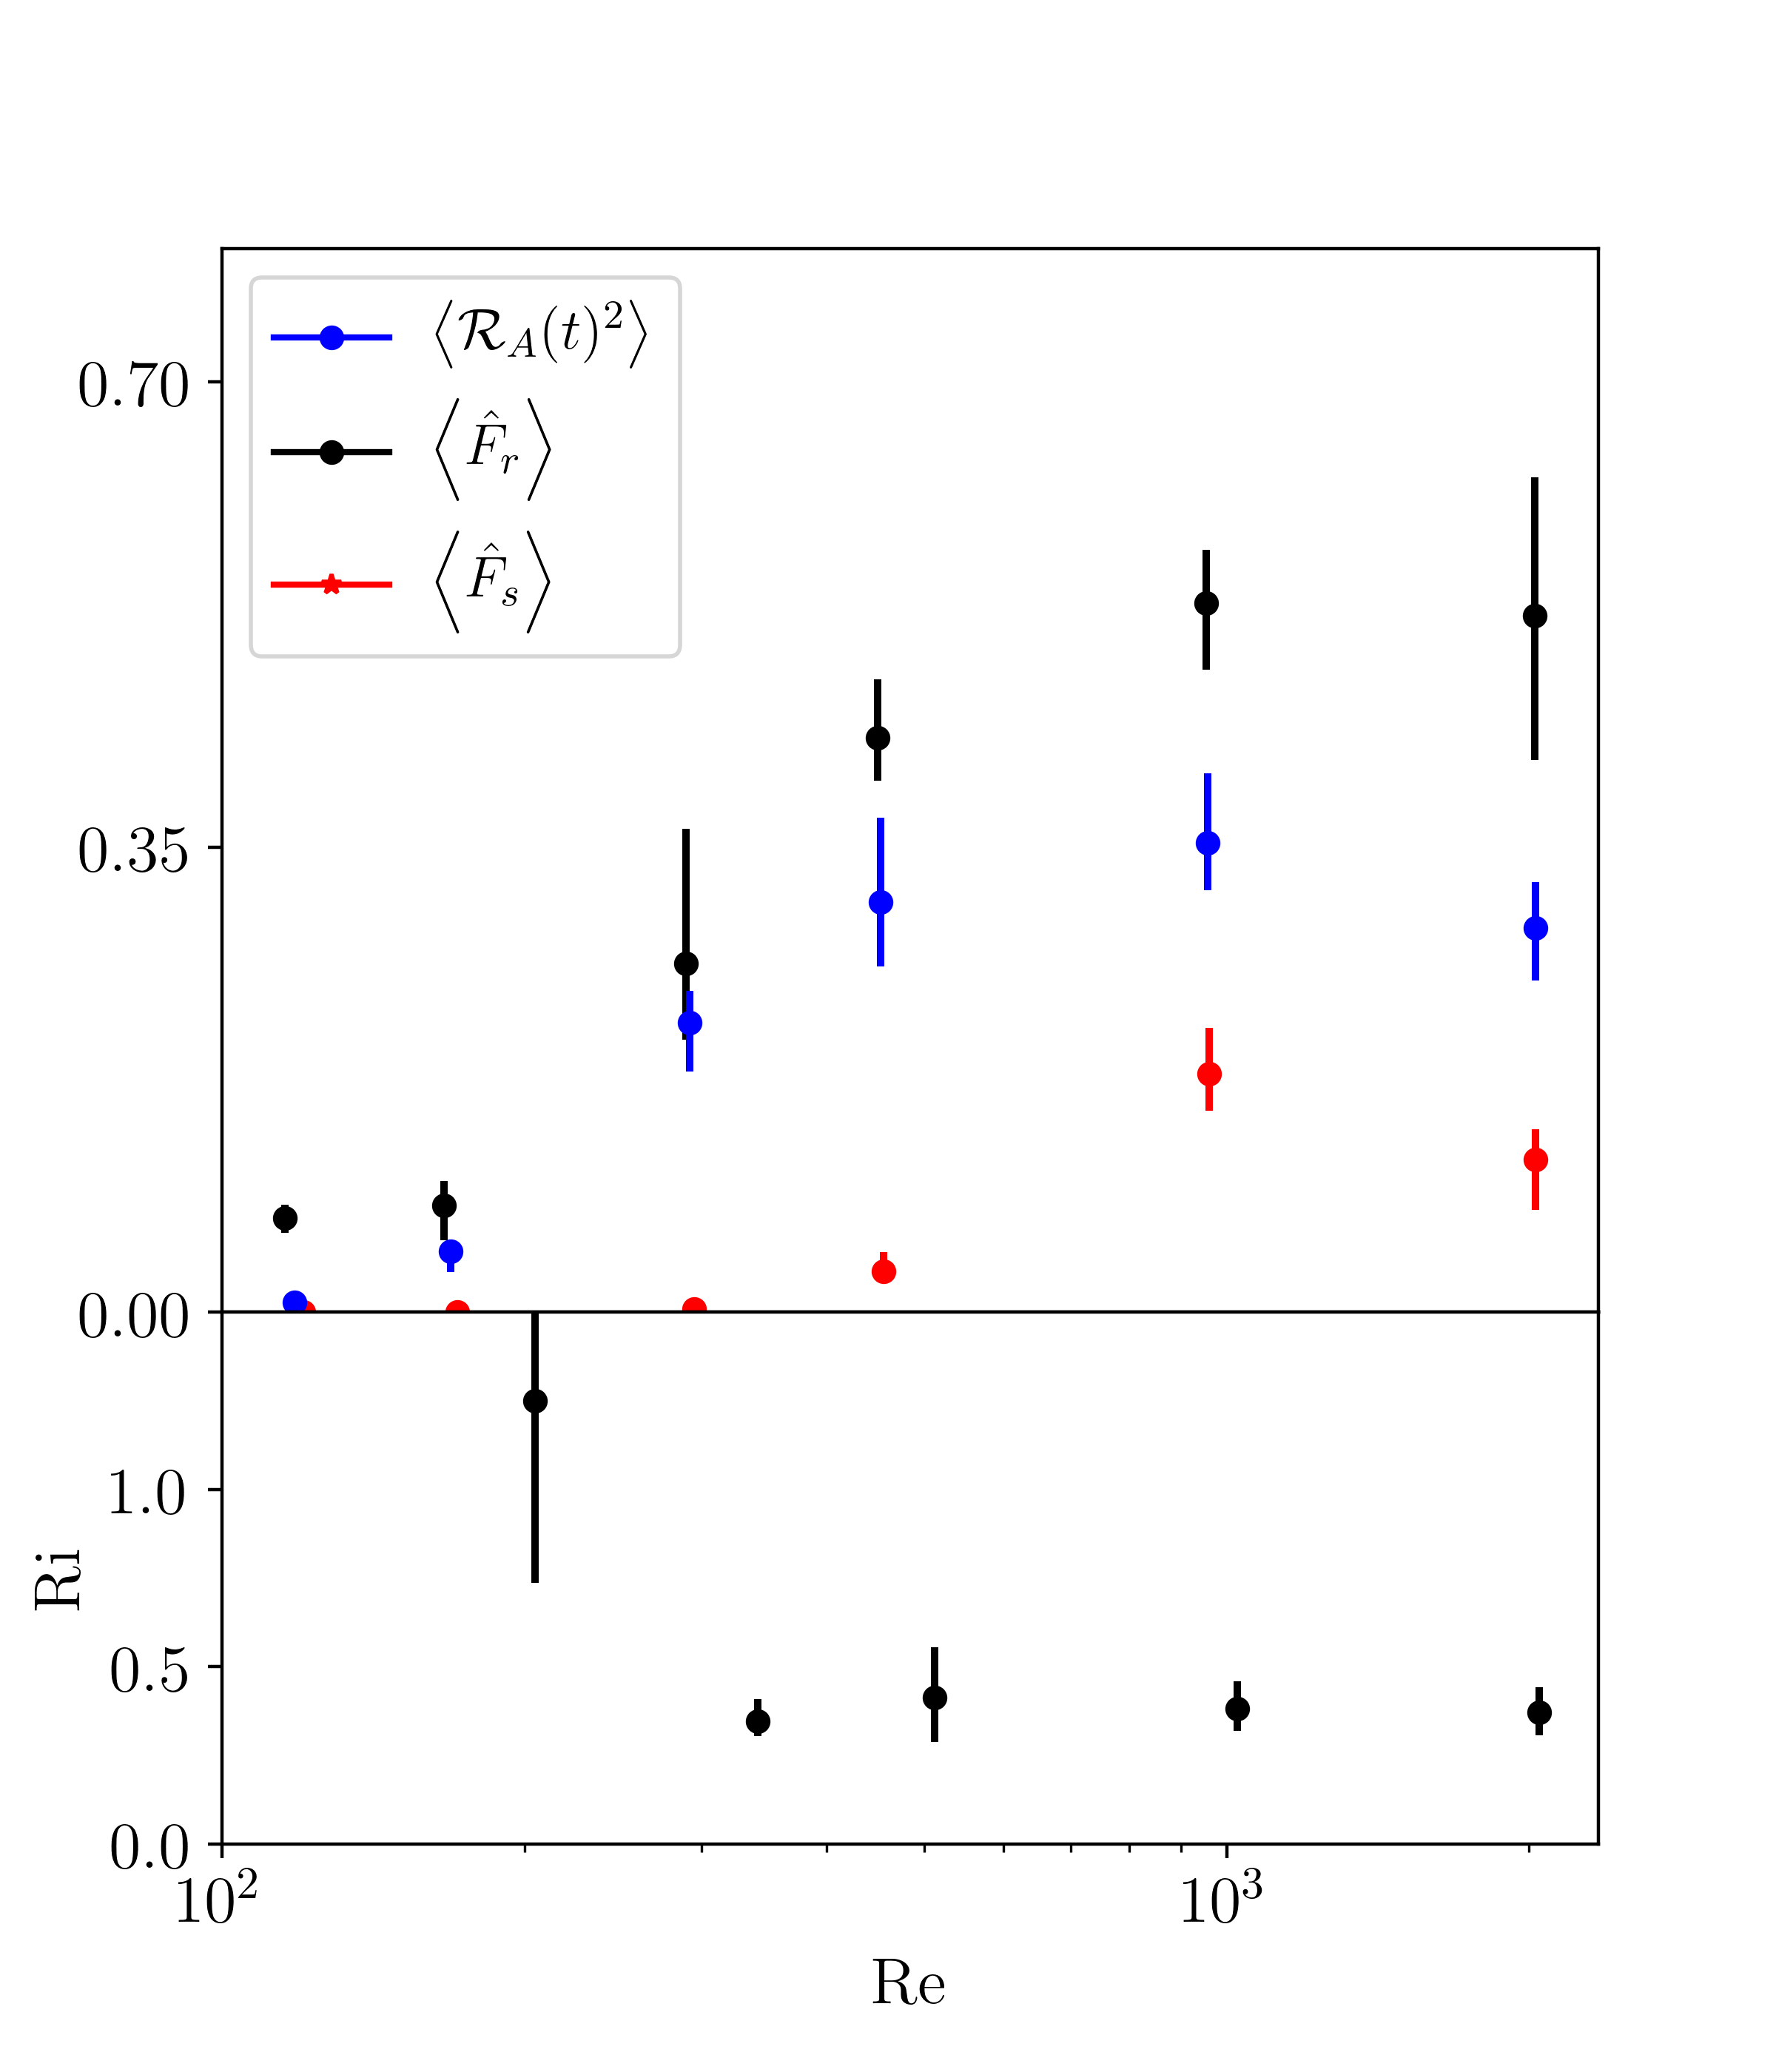
\includegraphics[width=\columnwidth]{plots/agg.png}
    \caption{Convergence w/ all runs}\label{fig:agg}
\end{figure}

\subsection{Applicability to Astrophysical Systems}

% magnetic winding, radiative diffusivity + effective Re. Might be applicable to
% inwards focusing too

Discussion foo

\section{Acknowledgements}\label{s:ack}

\bibliographystyle{mnras}
\bibliography{paper}

\clearpage
\onecolumn
\appendix

\section{Equation Implementations}\label{ss:strat_impl}

We denote $x \in [0, L_x], z \in [0, L_z]$ the simulation domain and $N_x, N_z$
the number of spectral modes in the respective dimensions. We perform direct
numerical simulation of \autoref{eq:vol_drive} with the open-source
pseudo-spectral code Dedalus (CITE).

Numerically, the nonlinear $\frac{\vec{\nabla}P}{\rho}$ term is problematic: we
desire a system where the fluid fields are not divided by one another. We
introduce $\varpi = \frac{P}{\rho}$ instead, then mandate $\rho_0, \varpi_0$
background fields satisfy hydrostatic equilibrium $\vec{\nabla}\varpi_0 +
\varpi_0 \vec{\nabla}\rho_0 + g\hat{z} = 0$. Taking isothermal stratification,
we find $\varpi_0 = gH$. We further change variables to $\Upsilon = \ln \rho -
\ln \rho_0$ and $\varpi_1 = \varpi - \varpi_0$ deviations from the background
state to obtain a system of equations at most quadratic in fluid fields:
\begin{subequations}\label{se:nl_var}
    \begin{align}
        \vec{\nabla} \cdot \vec{u} &= 0,\\
        \pd{\Upsilon}{t} + \p{\vec{u} \cdot \vec{\nabla}} \Upsilon
            - \frac{u_z}{H} &= 0,\\
        \pd{u_x}{t} + \p{\vec{u} \cdot \vec{\nabla}}u_x
            + \pd{\varpi_1}{x} + gH\pd{\Upsilon}{x}
            + \varpi_1 \pd{\Upsilon}{x} &= 0,\\
        \pd{u_z}{t} + \p{\vec{u} \cdot \vec{\nabla}}u_z
            + \pd{\varpi_1}{z} + gH\pd{\Upsilon}{z}
            + \varpi_1 \pd{\Upsilon}{z} - \frac{\varpi_1}{H} &= 0.
    \end{align}
\end{subequations}
It bears noting that these equations are exactly equivalent to the original
Euler equations and hence conserve horizontal momentum.

\subsection{Artificial Dissipation}

The nonlinear terms in the above equations will transfer energy from lower
wavenumbers to higher wavenumbers. Since spectral codes have no numerical
dissipation, artificial dissipation must be added. To ensure the dissipitive
system conserves horizontal momentum, we begin by adding dissipitive terms to
the flux-conservative form of the Euler fluid equations \autoref{se:nl_orig} (we
use stress tensor $\tau_{ij} = P\delta_{ij}$):
\begin{subequations}
    \begin{align}
        \vec{\nabla} \cdot \vec{u} &= 0,\\
        \partial_t \rho + \vec{\nabla} \cdot (\rho \vec{u} - \nu
            \vec{\nabla}(\rho - \rho_0)) &= 0,\label{eq:visc_cons_mom}\\
        \partial_t (\rho \vec{u}) + \vec{\nabla} \cdot (\rho \vec{u} \vec{u} +
            \mathrm{diag}(\rho \varpi) - \nu \rho \vec{\nabla}\vec{u}) + \rho g
            \hat{z} &= 0.
    \end{align}
\end{subequations}
The same $\nu$ is used for both the diffusive and viscous term, though this is
not required. Since the dissipation is not physical and is purely used for
numerical stability, we choose it such that hydrostatic equilibrium is not
modified. Some algebraic manipulation to re-cast it in the form of
\autoref{se:nl_var} gives
\begin{subequations}
    \begin{align}
        \vec{\nabla} \cdot \vec{u} &= 0,\\
        \partial_t \Upsilon + \p{\vec{u} \cdot \vec{\nabla}} \Upsilon -
            \frac{u_z}{H} - \nu\p{\nabla^2 \Upsilon + \p{\vec{\nabla}
            \Upsilon} \cdot \p{\vec{\nabla}\Upsilon} - \frac{2}{H}\partial_z
            \Upsilon + \frac{1 - e^{-\Upsilon}}{H^2}} &= 0,\\
        \partial_t \vec{u} + \p{\vec{u} \cdot \vec{\nabla}}\vec{u} +
            \vec{\nabla} \varpi + \varpi \vec{\nabla} \Upsilon - \nu \nabla^2
            \vec{u} + \vec{u} \nu\p{\nabla^2 \Upsilon + \p{\vec{\nabla}
            \Upsilon} \cdot \p{\vec{\nabla}\Upsilon} - \frac{2}{H}\partial_z
            \Upsilon + \frac{1 - e^{-\Upsilon}}{H^2}}&{}\nonumber\\
        - 2\nu \p{\p{\p{\vec{\nabla}\Upsilon} \cdot \vec{\nabla}}\vec{u} -
            \frac{1}{H}\partial_z \vec{u}} - \frac{\varpi_1}{H} &= 0.
    \end{align}
\end{subequations}
Hydrostatic equilibrium is still $\vec{\nabla} \varpi_0 + g\hat{z} = 0$ where
$\rho = \rho_0, \vec{u} = 0$. Including the damping layers and forcing terms as
described in \autoref{ss:numerics}, we finally obtain the full system of
equations as simulated in Dedalus:
\begin{subequations}
    \begin{align}
        \vec{\nabla} \cdot \vec{u} ={}& 0,\\
        \partial_t \Upsilon - \frac{u_z}{H}
            ={}& \nu\p{\nabla^2 \Upsilon + \p{\vec{\nabla}
            \Upsilon} \cdot \p{\vec{\nabla}\Upsilon} - \frac{2}{H}\partial_z
            \Upsilon + \frac{1 - e^{-\Upsilon}}{H^2}},\nonumber\\
            & - \p{\vec{u} \cdot \vec{\nabla}}\Upsilon
                -\Gamma(z) \Upsilon
                + \frac{F}{\rho_0(z)}e^{-\frac{(z - z_0)^2}{2\sigma^2}}
                    \cos \p{k_xx - \omega t},\\
        \pd{u_x}{t} + \pd{T}{x} + gH\pd{\Upsilon}{x} ={}&
            \nu \nabla^2 u_x
            - u_x \nu\p{\nabla^2 \Upsilon + \p{\vec{\nabla} \Upsilon} \cdot
                \p{\vec{\nabla}\Upsilon} - \frac{2}{H}\partial_z \Upsilon
                + \frac{1 - e^{-\Upsilon}}{H^2}}\nonumber\\
            &+ 2\nu \p{\p{\p{\vec{\nabla}\Upsilon} \cdot \vec{\nabla}}u_x
                - \frac{1}{H}\partial_z u_x}
            -\Gamma(z) u_x
                - \p{\vec{u} \cdot \vec{\nabla}}u_x
                - T_1 \pd{\Upsilon}{x},\\
        \pd{u_z}{t} + \pd{T}{z} + gH\pd{\Upsilon}{z} - \frac{T_1}{H} ={}&
            \nu \nabla^2 u_z
            - u_z \nu\p{\nabla^2 \Upsilon + \p{\vec{\nabla} \Upsilon} \cdot
                \p{\vec{\nabla}\Upsilon} - \frac{2}{H}\partial_z \Upsilon
                + \frac{1 - e^{-\Upsilon}}{H^2}}\nonumber\\
            &+ 2\nu \p{\p{\p{\vec{\nabla}\Upsilon} \cdot \vec{\nabla}}u_z -
                \frac{1}{H}\partial_z u_{z}}
            -\Gamma(z) u_z - \p{\vec{u} \cdot \vec{\nabla}}u_z
            - T_1 \pd{\Upsilon}{z}.
    \end{align}
\end{subequations}
\label{lastpage} % chktex 24
\end{document}
